% If you intend to adapt the material in this textbook
% in any way, then you must set the \adaptername and
% \adapteremail commands on lines 13 and 14 of this file
% to your full name and email address, respectively.
%
% Example usage:
% \newcommand{\adaptername}{Exampleface McLastname}
% \newcommand{\adapteremail}{exampleface-mclastname@example.web}
%
% Any duplications, derivations or adaptations of this work
% must be released under the Creative Commons BY-SA 4.0 licence.

\newcommand{\adaptername}{Teaching Team Bewijzen in de Wiskunde at Utrecht University} % Your full name
\newcommand{\adapteremail}{p.j.otte@uu.nl} % Your email address

% Page layout
% 0:6"x9", 1:a4, 2:usletter, 3:tablet, 4:phone
\newcounter{bookformat}\setcounter{bookformat}{1}

% Book version - if you are adapting the book, please leave
% these unchanged so that the original version can be traced.
\newcounter{versionmajor}\setcounter{versionmajor}{1}
\newcounter{versionminor}\setcounter{versionminor}{0}
\newcounter{versionpatch}\setcounter{versionpatch}{-1}
%Changed 0 to 1 to get a stable build version
\newcounter{versionstable}\setcounter{versionstable}{1}

\documentclass[10pt]{book}

% Includes
% !TeX root = ../../infdesc.tex
% !TeX root = ../../infdesc.tex

%
% Packages to be included
%

\usepackage{amsmath}
\usepackage{amsfonts}
\usepackage{amssymb}
\usepackage{amsthm}
\usepackage{afterpage}
\usepackage{appendix}
\usepackage{array}
\usepackage[british]{babel}
\usepackage{bbm}
\usepackage{bussproofs}
\usepackage{calc}
\usepackage{datetime}
    \newdateformat{customdate}{\dayofweekname{\THEDAY}{\THEMONTH}{\THEYEAR} \ordinaldate{\THEDAY} \monthname[\THEMONTH] \THEYEAR}
\usepackage{enumerate}
\usepackage[shortlabels]{enumitem}
\usepackage{environ}
\usepackage{fancyhdr}
\usepackage{float}
\usepackage[T1]{fontenc}
\usepackage[showcrop]{geometry}
\usepackage{graphicx}
\usepackage[hang,flushmargin]{footmisc}
\usepackage[utf8]{inputenc}
\usepackage{lastpage}
\usepackage{listings} % TeX code in TeX
    \lstset
    {
        language=[LaTeX]TeX,
        breaklines=true,
        basicstyle=\tt\color[HTML]{003388},
        keywordstyle=\color[HTML]{003388},
        emphstyle=\color[HTML]{003388},
        identifierstyle=\color[HTML]{003388},
        commentstyle=\color[HTML]{883300},
        escapeinside={(*@}{@*)},
        escapebegin={@*)},
        emph={includegraphics,maketitle,setlength,text,theoremstyle},
    }
\usepackage{mathptmx}
\usepackage[framemethod=TikZ]{mdframed}
\usepackage{multicol}
\usepackage{pdfpages}
\usepackage{pifont}
\usepackage{refcount}
\usepackage[absolute]{textpos}
    \setlength{\TPHorizModule}{1in}
    \setlength{\TPVertModule}{1in}
\usepackage[artemisia]{textgreek}
\usepackage{thmtools}
\usepackage{thm-restate}
\usepackage{tikz}
    \tikzset{node distance=3cm and 5cm, auto}
    \usetikzlibrary{arrows,shapes,decorations.pathreplacing}
\usepackage{tikz-cd}
\usepackage{titlesec}
\usepackage{type1cm}
\usepackage[normalem]{ulem}
\usepackage{xcolor}
\usepackage{etoolbox}
\usepackage{ifthen}
\usepackage{xpatch}

% Packages that are fussy about what order they're put in
\usepackage[makeindex]{imakeidx}
\usepackage{hyperref}
\usepackage[numbered]{bookmark}
    \hypersetup{
        pdftitle={An Infinite Descent into Pure Mathematics},
        pdfsubject={Introductory pure mathematics textbook with an emphasis on proof},
        pdfauthor={Clive Newstead},
        pdfkeywords={math,maths,mathematics,pure mathematics,undergraduate,textbook},
        pdfproducer={Clive Newstead},
        pdfcreator={LaTeX}
    }
\usepackage[nameinlink,capitalise]{cleveref}
    \crefrangelabelformat{section}{#3#1#4--#5#2#6}

% !TeX root = ../../infdesc.tex

%
% Custom symbols and commands
%

% Text mode

% Contact and website information
\newcommand{\authoremail}{clive.newstead@infinitedescent.xyz}
\newcommand{\bookurl}{https://infinitedescent.xyz}

% Symbols for optional content
\newcommand{\optmarksymbol}{$\star$}
\newcommand{\optmark}[1]{\optmarksymbol~#1}

% Indicators of where AC is used
\newcommand{\assumesAC}[1]{\textsuperscript{\hyperref[axChoice]{\color{#1}\textbf{AC}}}}

% QED symbols
\newcommand{\nonproofqedsymbol}{$\vartriangleleft$}
\newcommand{\defqedsymbol}{\color{defqedcol} $\vartriangleleft$}
\newcommand{\exqedsymbol}{\color{exqedcol} $\vartriangleleft$}
\newcommand{\prqedsymbol}{\color{prqedcol} $\vartriangleleft$}
\newcommand{\tipqedsymbol}{\color{tipqedcol} $\vartriangleleft$}
\newcommand{\quoteqedsymbol}{\color{excol} \ding{126}}

% Symbols for theorem environments
\newcommand{\defintrosymbol}{\ding{70}\hspace{4pt}} % Star
\newlength{\defsymbolwidth}
\setlength{\defsymbolwidth}{\widthof{\defintrosymbol}}
% \addtolength{\defsymbolwidth}{1pt}

\newcommand{\thmintrosymbol}{\ding{67}\hspace{4pt}} % Plus
\newlength{\thmsymbolwidth}
\setlength{\thmsymbolwidth}{\widthof{\thmintrosymbol}}
% \addtolength{\thmsymbolwidth}{1pt}

\newcommand{\exintrosymbol}{\ding{48}\hspace{4pt}} % Pen up
\newlength{\exsymbolwidth}
\setlength{\exsymbolwidth}{\widthof{\exintrosymbol}}
% \addtolength{\exsymbolwidth}{1pt}

\newcommand{\printrosymbol}{\ding{46}\hspace{4pt}} % Pen down
\newlength{\prsymbolwidth}
\setlength{\prsymbolwidth}{\widthof{\printrosymbol}}
% \addtolength{\prsymbolwidth}{1pt}

\newcommand{\tipintrosymbol}{\ding{118}\hspace{4pt}} % Four diamonds
\newlength{\tipsymbolwidth}
\setlength{\tipsymbolwidth}{\widthof{\tipintrosymbol}}
% \addtolength{\tipsymbolwidth}{1pt}

\newcommand{\quoteintrosymbol}{\ding{125}\hspace{4pt}} % Open quotation mark
\newlength{\quotesymbolwidth}
\setlength{\quotesymbolwidth}{\widthof{\quoteintrosymbol}}
% \addtolength{\quotesymbolwidth}{1pt}

% For scaling figures that might overflow with small page sizes
\newcommand{\fitwidth}[1]{\resizebox{\textwidth}{!}{#1}}
\newcommand{\fitwidthc}[2]{\resizebox{#1\textwidth}{!}{#2}}
\newcommand{\fitheight}[1]{\resizebox{\textheight}{!}{#1}}
\newcommand{\fitheightc}[2]{\resizebox{#1\textheight}{!}{#2}}

% To-do remarks
\newcommand{\todo}[1]{{\color{magenta} \textbf{Note:} #1}}

% Custom table alignments
% Source: http://tex.stackexchange.com/questions/12703/
\newcolumntype{L}[1]{>{\raggedright\let\newline\\\arraybackslash\hspace{0pt}}m{#1}}
\newcolumntype{C}[1]{>{\centering\let\newline\\\arraybackslash\hspace{0pt}}m{#1}}
\newcolumntype{R}[1]{>{\raggedleft\let\newline\\\arraybackslash\hspace{0pt}}m{#1}}

% Truth table shortcuts
\newcommand{\TT}{{\color{truecol}\checkmark}}
\newcommand{\FF}{${\color{falsecol}\times}$}

% Emphasis in extracts
% \newcommand{\xtremph}[1]{\!\fcolorbox{black}{indbasecol}{\!#1\!}}
\newcommand{\xtremph}[1]{\!\colorbox{indbasecol}{\!#1\!}}

% Source for extracts
\newcommand{\xtrsource}[1]{taken from #1}

% Commands for proof-writing section
\newcommand{\vtinstructions}[1]{${\color{defcol} \langle \text{#1} \rangle}$}
\newcommand{\propproof}[1]{\vtinstructions{insert proof of #1 here}}
\newcommand{\propstate}[1]{\vtinstructions{state #1 here}}
\newcommand{\propcite}[1]{\vtinstructions{cite #1 here}}
\newcommand{\vardefine}[1]{\vtinstructions{define #1 here}}
\newcommand{\vtor}{\hspace{7pt}--- \textit{or} ---}

\newenvironment{vocabtemplate}{\begin{minipage}{0.05\linewidth}~\end{minipage}\vline\hspace{7pt}\begin{minipage}{0.9\linewidth}}{\end{minipage}}

\newenvironment{snippet}{\begin{minipage}[b]{7pt}~\end{minipage}\vline\hspace{7pt}\begin{minipage}[b]{0.88\linewidth}}{\end{minipage}}

% Warning messages for incomplete sections
\newcommand{\chexwarning}{%
    \begin{figure}[H]\centering {\Large \color{red} \textbf{Under construction!}} \\
    The end-of-chapter exercise sections are new and in an incomplete state.\end{figure}%
}
\newcommand{\incomplete}{%
    \begin{figure}[H]\centering {\Large \color{red} \textbf{Warning!}} \\
    This section is not yet finished---do not rely on its correctness or completeness.\end{figure}%
}
\newcommand{\incompletefromhere}{%
    \begin{figure}[H]\centering {\Large \color{red} \textbf{Warning!}} \\
    The section beyond this point is not yet finished---do not rely on its correctness or completeness.\end{figure}%
}

% Instructions for true-false and always-sometimes-never questions
\newcommand{\tfquestiontext}[2]{%
In \Crefrange{#1}{#2}, determine (with proof) whether the statement is true or false.
}
\newcommand{\asnquestiontext}[2]{%
In \Crefrange{#1}{#2}, determine (with proof) whether the conclusion is always, sometimes or never true under the given hypotheses.
}



% Math mode

% Custom quantifiers
\newcommand{\forQ}{\mathbin{\text{\raisebox{1.1pt}{\rotatebox[origin=c]{180}{$\mathsf{Q}$}}}}} % Rotated Q

% Introduction and elimination rule labels
\newcommand{\introrule}[1]{($#1$\textsc{i})}
\newcommand{\introrulesub}[2]{($#1$\textsc{i}$_{#2}$)}
\newcommand{\elimrule}[1]{($#1$\textsc{e})}
\newcommand{\elimrulesub}[2]{($#1$\textsc{e}$_{#2}$)}

% Rotated 'leads to' arrow for proof trees
\newcommand{\downleadsto}{\mathbin{\text{\rotatebox{-90}{$\leadsto$}}}}
\newcommand{\upleadsto}{\mathbin{\text{\rotatebox{90}{$\leadsto$}}}}
\newcommand{\leftleadsto}{\mathbin{\text{\rotatebox{180}{$\leadsto$}}}}

% String diagrams for inductively defined sets
\newcommand{\sdconstructor}[2]{node[circle, draw, text width=10, text centered, fill=indbasecol](#1) {#2}}

% Diagrams for homogeneous relations
\newcommand{\relnode}[2]{node[circle, draw, text width=10, text centered](#1) {#2}}

% Tagged step in proof tree
\newcommand{\TagC}[1]{\RightLabel{\scriptsize #1}}

% Custom binary operations
\newcommand{\symmdiff}{\mathbin{\triangle}}

% Vertical bar for use with \left ... \right (e.g. for set-builder notation)
\newcommand{\middlemid}{~\middle|~}

% Symbol for binary operations
\newcommand{\binop}{\star}
\newcommand{\binopalt}{\diamond}

% Modifications to default symbols
\renewcommand{\labelitemii}{$\diamond$}
\renewcommand{\le}{\leqslant}
\renewcommand{\leq}{\leqslant}
\renewcommand{\preceq}{\preccurlyeq}
\renewcommand{\ge}{\geqslant}
\renewcommand{\geq}{\geqslant}
\renewcommand*{\thefootnote}{\color{fncol} [\alph{footnote}]}

% Modular arithmetic
\newcommand{\cmod}[1]{~\left(\text{mod}~#1\right)}

% Force \displaystyle for indexed operations
\let\nsum\sum
\let\nprod\prod
\let\nbigcap\bigcap
\let\nbigcup\bigcup
\let\nbigsqcup\bigsqcup
\let\nbigwedge\bigwedge
\let\nbigvee\bigvee

\renewcommand{\sum}{\displaystyle\nsum}
\renewcommand{\prod}{\displaystyle\nprod}
\renewcommand{\bigcap}{\displaystyle\nbigcap}
\renewcommand{\bigcup}{\displaystyle\nbigcup}
\renewcommand{\bigsqcup}{\displaystyle\nbigsqcup}
\renewcommand{\bigwedge}{\displaystyle\nbigwedge}
\renewcommand{\bigvee}{\displaystyle\nbigvee}

\newcommand{\ssum}{\nsum\limits}
\newcommand{\sprod}{\prod\limits}
\newcommand{\sbigcap}{\nbigcap\limits}
\newcommand{\sbigcup}{\nbigcup\limits}
\newcommand{\sbigsqcup}{\nbigsqcup\limits}


% Text and math mode

% Superscripts for ordinal numbers (1st, 2nd, 3rd, 4th, ...)
\newcommand{\supst}{\textsuperscript{st}}
\newcommand{\supnd}{\textsuperscript{nd}}
\newcommand{\suprd}{\textsuperscript{rd}}
\newcommand{\supth}{\textsuperscript{th}}




%
% Modifications for derivations
%

\newcommand{\ifadaptedelse}[2]{\ifdefempty{\adaptername}{#2}{#1}}
\newcommand{\ifadapted}[1]{\ifadaptedelse{#1}{}}
\newcommand{\iforiginal}[1]{\ifadaptedelse{}{#1}}




%
% Language
%

\newcommand{\gbus}[2]{%
\ifnumequal{\value{englishvariant}}{0}{#1}{}%
\ifnumequal{\value{englishvariant}}{1}{#2}{}%
}
\input{book/includes/organisation.tex}
% !TeX root = ../../infdesc.tex

%
% Paper size configuration
%

% Default values for watermark location
\newcommand{\watermarkh}{0in}
\newcommand{\watermarkv}{0in}

% Print version (6x9, no crops)
\ifnumequal{\value{bookformat}}{0}{%
    \geometry{
        paperwidth={6in},
        paperheight={9in},
        margin={0.5in},
        bindingoffset={0.2in},
        includehead,
        includefoot,
        centering
    }
    \setlength{\leftmargini}{0.25in}
    \setlength{\leftmarginii}{0.25in}
    \setlength{\leftmarginiii}{0.25in}
    \renewcommand{\watermarkh}{5in}
    \renewcommand{\watermarkv}{8in}
    \hypersetup{pdfpagelayout={TwoPageRight}}
}

% Print version (6x9 on letter paper, with crops)
\ifnumequal{\value{bookformat}}{100}{%
    \geometry{
        paper={letterpaper},
        layoutwidth={6in},
        layoutheight={9in},
        layouthoffset={1.25in},
        layoutvoffset={1in},
        margin={0.5in},
        bindingoffset={0.2in},
        includehead,
        includefoot,
        centering
    }
    \setlength{\leftmargini}{0.25in}
    \setlength{\leftmarginii}{0.25in}
    \setlength{\leftmarginiii}{0.25in}
    \renewcommand{\watermarkh}{6.25in}
    \renewcommand{\watermarkv}{9in}
    \hypersetup{pdfpagelayout={TwoPageRight}}
}

% A4 paper
\ifnumequal{\value{bookformat}}{1}{%
    \geometry{
        paper={a4paper},
        margin={25mm},
        marginratio={1:1},
        includehead,
        includefoot
    }
    \renewcommand{\watermarkh}{185mm}
    \renewcommand{\watermarkv}{272mm}
    \hypersetup{pdfpagelayout={OneColumn}}
}

% US letter
\ifnumequal{\value{bookformat}}{2}{%
    \geometry{
        paper={letterpaper},
        margin={1in},
        marginratio={1:1},
        includehead,
        includefoot
    }
    \renewcommand{\watermarkh}{7.5in}
    \renewcommand{\watermarkv}{10in}
    \hypersetup{pdfpagelayout={OneColumn}}
}

% Tablet version
\ifnumequal{\value{bookformat}}{3}{%
    \geometry{
        paperwidth={150mm},
        paperheight={240mm},
        margin={0.5cm},
        marginratio={1:1},
        includehead,
        includefoot
    }
    \renewcommand{\watermarkh}{125mm}
    \renewcommand{\watermarkv}{215mm}
    \hypersetup{pdfpagelayout={SinglePage}}
}

% Phone version
\ifnumequal{\value{bookformat}}{4}{%
    \geometry{
        paperwidth={130mm},
        paperheight={230mm},
        margin={5mm},
        marginratio={1:1},
        includehead,
        includefoot
    }
    \renewcommand{\watermarkh}{105mm}
    \renewcommand{\watermarkv}{205mm}
    \setlength{\leftmargini}{0.5cm}
    \setlength{\leftmarginii}{0.5cm}
    \setlength{\leftmarginiii}{0.5cm}
    \hypersetup{pdfpagelayout={SinglePage}}
}

% Watermark for preview versions

\iforiginal{%
\ifnumgreater{0}{\value{versionpatch}}{%
    \usepackage{draftwatermark}
        \SetWatermarkHorCenter{\watermarkh}
        \SetWatermarkVerCenter{\watermarkv}
        \SetWatermarkLightness{0.9}
        \SetWatermarkText{\texttt{preview}}
}}





%
% Document formatting
%

% Lengths and spacing

\setlength{\parindent}{0pt}
\setlength{\parskip}{10pt}
\setlist{topsep=0pt,leftmargin=*}

% Source: http://tex.stackexchange.com/questions/22119/
\makeatletter
\def\thm@space@setup{%
  \thm@preskip=\parskip
  \thm@postskip=0pt
}
\makeatother

% Better paragraph and list spacing inside theorem environments
% If theorem boxes look strange (e.g. too much whitespace, title overlaps with border), swap the commenting of the two lines below
\newcommand{\fixthmbox}{\setlist[itemize,enumerate]{topsep={5pt},leftmargin=*}\setlength{\parskip}{7pt}}
%\newcommand{\fixthmbox}{\setlist[itemize,enumerate]{topsep={5pt},leftmargin=*}\setlength{\parskip}{7pt}\vspace{-7pt}}

% Better spacing when a theorem environment begins or ends with a list
\newcommand{\fixlistskip}{~ \vspace{-20pt}}

% Avoid breaking mid-formula
\relpenalty=9999
\binoppenalty=9999

% Reduce hyphenation.
% Source: https://ctan.org/tex-archive/info/l2tabu/english/
\tolerance 1414
\hbadness 1414
\emergencystretch 1.5em
\hfuzz 0.3pt
\widowpenalty=10000
\vfuzz \hfuzz
\raggedbottom



% Header and footer styles

\pagestyle{fancy}
\fancyhf{}
\setlength{\headheight}{14pt}

\renewcommand{\sectionmark}[1]{\markboth{\leftmark}{Section \thesection.\ #1}}
\renewcommand{\chaptermark}[1]{\markboth{Chapter \thechapter.\ #1}{\rightmark}}
\renewcommand{\headrulewidth}{0pt}
\renewcommand{\footrulewidth}{0pt}

\fancyhead[RE]{{\color{hdcol}\fontfamily{bch}\itshape \nouppercase{\leftmark}}}
\fancyhead[LO]{{\color{hdcol}\fontfamily{bch}\itshape \nouppercase{\rightmark}}}
\fancyhead[RO,LE]{\thepage}
\fancyfoot[C]{\thepage}



% Chapter and section title styles styles

\makeatletter
\titleformat{\chapter}[display]{\LARGE}{\color{midgray} \@chapapp\ \thechapter}{0pt}{\fontfamily{bch}\Huge\bfseries}
\titleformat{\section}[display]{\Large}{\color{midgray} Section \thesection}{-10pt}{\fontfamily{bch}\LARGE\bfseries}
\makeatother





%
% Colours
%

% For theorem environments

% Results
\definecolor{thmcol}{HTML}{002882}
\definecolor{thmcolac}{HTML}{6699CC}
\definecolor{thmbdcol}{HTML}{77AADD}
\definecolor{thmbgcol}{HTML}{F7FCFF}

% Definitions
\definecolor{defcol}{HTML}{820028}
\definecolor{defcolac}{HTML}{CC6699}
\definecolor{defbdcol}{HTML}{DD77AA}
\definecolor{defbgcol}{HTML}{FFF7FC}
\definecolor{defqedcol}{HTML}{820028}

% Examples
\definecolor{excol}{HTML}{006644}
\definecolor{excolac}{HTML}{66CCCC}
\definecolor{exbdcol}{HTML}{888888}
\definecolor{exbgcol}{HTML}{FCFCFC}
\definecolor{exqedcol}{HTML}{666666}

% Exercises
\definecolor{prcol}{HTML}{884400}
\definecolor{prbdcol}{HTML}{CCCC66}
\definecolor{prbgcol}{HTML}{FCFCFC}
\definecolor{prqedcol}{HTML}{666666}

% Proofs
\definecolor{pfcol}{HTML}{555555}

% Tips
\definecolor{tipcol}{HTML}{550055}
\definecolor{tipcolac}{HTML}{CC66CC}
\definecolor{tipbdcol}{HTML}{AA77DD}
\definecolor{tipbgcol}{HTML}{FCF7FF}
\definecolor{tipqedcol}{HTML}{990099}

% Optional content 
\definecolor{optmarkcol}{HTML}{770077}

% Other colours

\definecolor{notecol}{HTML}{2266AA}
\definecolor{citecol}{HTML}{883388}
\definecolor{refcol}{HTML}{115588}
\definecolor{urlcol}{HTML}{115588}
\definecolor{truecol}{HTML}{000000}  % Colour of \TT 'true' symbol in truth tables
\definecolor{falsecol}{HTML}{AA2200} % Colour of \FF 'false' symbol in truth tables

% Colours for links and so on
\hypersetup{
    colorlinks=true,
    linkcolor={refcol},
    citecolor={citecol},
    urlcolor={urlcol}
}

% For proof by induction diagrams
\definecolor{indstepcol}{HTML}{FFF0F8}
\definecolor{indbasecol}{HTML}{DDEEFF}

% New colours for the infinity symbols on the title page
\definecolor{infty1}{HTML}{880088}
\definecolor{infty2}{HTML}{000088}
\definecolor{infty3}{HTML}{008888}
\definecolor{infty4}{HTML}{008800}
\definecolor{infty5}{HTML}{888800}
\definecolor{infty6}{HTML}{880000}
\definecolor{infty7}{HTML}{880088}
\definecolor{infty8}{HTML}{888888}

% Miscellaneous colours
\definecolor{lccol1}{HTML}{3333CC}    % Light blue
\definecolor{lccol2}{HTML}{003388}    % Dark blue
\definecolor{gridlines}{HTML}{DDDDDD} % Light grey
\definecolor{midgray}{HTML}{777777}   % Mid grey
\definecolor{fncol}{HTML}{664466}     % Footnote labels
\definecolor{hdcol}{HTML}{444444}     % Headers
% !TeX root = ../../infdesc.tex

%
% Custom theorem environments
%

% Styles

% Width of border around shaded theorem boxes
\newcommand{\thmboxborderwidth}{0.25pt}

\declaretheoremstyle[
    spaceabove=6pt,
    spacebelow=6pt,
    headfont={\color{thmcol}\fontfamily{bch}\bfseries\hspace{-\thmsymbolwidth}\thmintrosymbol},
    headpunct={{\par\nobreak}\\},
    notefont={\mdseries},
    notebraces={(}{)},
    bodyfont=\normalfont
]{infdescthm}

\declaretheoremstyle[
    spaceabove=6pt,
    spacebelow=6pt,
    headfont={\color{thmcol}\fontfamily{bch}\bfseries\hspace{-\thmsymbolwidth}\thmintrosymbol},
    headpunct={{\par\nobreak}\\},
    notefont={\mdseries},
    notebraces={(}{)},
    bodyfont={\fixthmbox\normalfont},
    shaded={bgcolor=thmbgcol, rulecolor=thmbdcol, rulewidth=\thmboxborderwidth}
]{infdescimptthm}

\declaretheoremstyle[
    spaceabove=6pt,
    spacebelow=6pt,
    headfont={\color{defcol}\fontfamily{bch}\bfseries\hspace{-\defsymbolwidth}\defintrosymbol},
    headpunct={{\par\nobreak}\\},
    notefont={\mdseries},
    notebraces={(}{)},
    bodyfont=\normalfont
]{infdescdef}

\declaretheoremstyle[
    spaceabove=6pt,
    spacebelow=6pt,
    headfont={\color{defcol}\fontfamily{bch}\bfseries\hspace{-\defsymbolwidth}\defintrosymbol},
    headpunct={{\par\nobreak}\\},
    notefont={\mdseries},
    notebraces={(}{)},
    bodyfont={\fixthmbox\normalfont},
    shaded={bgcolor=defbgcol, rulecolor=defbdcol, rulewidth=\thmboxborderwidth}
]{infdescimptdef}

\declaretheoremstyle[
    spaceabove=6pt,
    spacebelow=6pt,
    headfont={\color{excol}\fontfamily{bch}\bfseries\hspace{-\exsymbolwidth}\exintrosymbol},
    headpunct={{\par\nobreak}\\},
    notefont={\mdseries},
    notebraces={(}{)},
    bodyfont=\normalfont,
    qed={\exqedsymbol}
]{infdescex}

\declaretheoremstyle[
    spaceabove=6pt,
    spacebelow=6pt,
    headfont={\color{excol}\fontfamily{bch}\bfseries\hspace{-\exsymbolwidth}\exintrosymbol},
    headpunct={{\par\nobreak}\\},
    notefont={\mdseries},
    notebraces={(}{)},
    bodyfont={\fixthmbox\normalfont},
    shaded={bgcolor=exbgcol, rulecolor=exbdcol, rulewidth=\thmboxborderwidth}
]{infdescimptex}

\declaretheoremstyle[
    spaceabove=6pt,
    spacebelow=6pt,
    headfont={\color{excol}\fontfamily{bch}\bfseries\hspace{-\quotesymbolwidth}\quoteintrosymbol},
    headpunct={{\par\nobreak}\\},
    notefont={\mdseries},
    notebraces={(}{)},
    bodyfont=\normalfont,
    qed={\quoteqedsymbol}
]{infdescquote}

\declaretheoremstyle[
    spaceabove=6pt,
    spacebelow=6pt,
    headfont={\color{prcol}\fontfamily{bch}\bfseries\hspace{-\prsymbolwidth}\printrosymbol},
    headpunct={{\par\nobreak}\\},
    notefont={\mdseries},
    notebraces={(}{)},
    bodyfont=\normalfont,
    qed={\exqedsymbol}
]{infdescpr}

\declaretheoremstyle[
    spaceabove=6pt,
    spacebelow=6pt,
    headfont={\color{prcol}\fontfamily{bch}\bfseries\hspace{-\prsymbolwidth}\printrosymbol},
    headpunct={{\par\nobreak}\\},
    notefont={\mdseries},
    notebraces={(}{)},
    bodyfont={\fixthmbox\normalfont},
    shaded={bgcolor=prbgcol, rulecolor=prbdcol, rulewidth=\thmboxborderwidth}
]{infdescimptpr}

\declaretheoremstyle[
    spaceabove=6pt,
    spacebelow=6pt,
    headfont={\color{midgray}\fontfamily{bch}\bfseries},
    headpunct={.},
    notefont={\mdseries},
    notebraces={(}{)},
    bodyfont=\normalfont
]{infdescchapex}

\declaretheoremstyle[
    spaceabove=6pt,
    spacebelow=6pt,
    headfont={\color{tipcol}\fontfamily{bch}\bfseries\hspace{-\tipsymbolwidth}\tipintrosymbol},
    headpunct={\par\nobreak\\},
    notefont={\mdseries},
    notebraces={(}{)},
    bodyfont=\normalfont,
    qed={\tipqedsymbol}
]{infdesctip}

\declaretheoremstyle[
    spaceabove=6pt,
    spacebelow=6pt,
    headfont={\color{tipcol}\fontfamily{bch}\bfseries\hspace{-\tipsymbolwidth}\tipintrosymbol},
    headpunct={\par\nobreak\\},
    notefont={\mdseries},
    notebraces={(}{)},
    bodyfont={\fixthmbox\normalfont},
    shaded={bgcolor=tipbgcol, rulecolor=tipbdcol, rulewidth=\thmboxborderwidth}
]{infdescimpttip}

\declaretheoremstyle[
    spaceabove=6pt,
    spacebelow=6pt,
    headfont={\color{pfcol}\fontfamily{bch}\bfseries\itshape},
    headpunct={\par\nobreak\\},
    notefont={\mdseries},
    notebraces={}{},
    bodyfont=\normalfont,
    qed={\color{pfcol}$\Box$}
]{infdescpf}

\declaretheoremstyle[
    spaceabove=6pt,
    spacebelow=6pt,
    headfont={\color{pfcol}\fontfamily{bch}\bfseries\itshape},
    headpunct={\par\nobreak\\},
    notefont={\mdseries},
    notebraces={}{},
    bodyfont=\normalfont
]{infdescpfnoqed}



% Results

\declaretheorem[style=infdescimptthm, numberwithin=section, Refname={Theorem,Theorems}, name=Theorem]{theorem}
\declaretheorem[style=infdescimptthm, sibling=theorem, Refname={Theorem,Theorems}, name={Theorem\assumesAC{thmcolac}}]{theoremac}
\declaretheorem[style=infdescimptthm, numberwithin=chapter, Refname={Theorem,Theorems}, name=Theorem]{chtheorem}
\declaretheorem[style=infdescimptthm, sibling=theorem, refname={theorem,theorems}, Refname={Theorem,Theorems}, name=Theorem]{itheorem}
\declaretheorem[style=infdescimptthm, numbered=no, refname={theorem,theorems}, Refname={Theorem,Theorems}, name=Theorem]{theorem*}
\declaretheorem[style=infdescimptthm, sibling=theorem, refname={theorem,theorems}, Refname={Theorem,Theorems}, name={\optmark{Theorem}}]{otheorem}

\declaretheorem[style=infdescthm, sibling=theorem, refname={lemma,lemmas}, Refname={Lemma,Lemmas}, name=Lemma]{lemma}
\declaretheorem[style=infdescthm, sibling=theorem, refname={lemma,lemmas}, Refname={Lemma,Lemmas}, name={Lemma\assumesAC{thmcolac}}]{lemmaac}
\declaretheorem[style=infdescthm, sibling=chtheorem, refname={lemma,lemmas}, Refname={Lemma,Lemmas}, name=Lemma]{chlemma}
\declaretheorem[style=infdescimptthm, sibling=theorem, refname={lemma,lemmas}, Refname={Lemma,Lemmas}, name=Lemma]{ilemma}
\declaretheorem[style=infdescthm, numbered=no, refname={lemma,lemmas}, Refname={Lemma,Lemmas}, name=Lemma]{lemma*}
\declaretheorem[style=infdescthm, sibling=theorem, refname={lemma,lemmas}, Refname={Lemma,Lemmas}, name={\optmark{Lemma}}]{olemma}

\declaretheorem[style=infdescthm, sibling=theorem, refname={proposition,propositions}, Refname={Proposition,Propositions}, name=Proposition]{proposition}
\declaretheorem[style=infdescthm, sibling=theorem, refname={proposition,propositions}, Refname={Proposition,Propositions}, name={Proposition\assumesAC{thmcolac}}]{propositionac}
\declaretheorem[style=infdescthm, sibling=chtheorem, refname={proposition,propositions}, Refname={Proposition,Propositions}, name=Proposition]{chproposition}
\declaretheorem[style=infdescimptthm, sibling=theorem, refname={proposition,propositions}, Refname={Proposition,Propositions}, name=Proposition]{iproposition}
\declaretheorem[style=infdescthm, numbered=no, refname={proposition,propositions}, Refname={Proposition,Propositions}, name=Proposition]{proposition*}
\declaretheorem[style=infdescthm, sibling=theorem, refname={proposition,propositions}, Refname={Proposition,Propositions}, name={\optmark{Proposition}}]{oproposition}

\declaretheorem[style=infdescthm, sibling=theorem, refname={corollary,corollaries}, Refname={Corollary,Corollaries}, name=Corollary]{corollary}
\declaretheorem[style=infdescthm, sibling=theorem, refname={corollary,corollaries}, Refname={Corollary,Corollaries}, name={Corollary\assumesAC{thmcolac}}]{corollaryac}
\declaretheorem[style=infdescthm, sibling=chtheorem, refname={corollary,corollaries}, Refname={Corollary,Corollaries}, name=Corollary]{chcorollary}
\declaretheorem[style=infdescimptthm, sibling=theorem, refname={corollary,corollaries}, Refname={Corollary,Corollaries}, name=Corollary]{icorollary}
\declaretheorem[style=infdescthm, numbered=no, refname={corollary,corollaries}, Refname={Corollary,Corollaries}, name=Corollary]{corollary*}
\declaretheorem[style=infdescthm, sibling=theorem, refname={corollary,corollaries}, Refname={Corollary,Corollaries}, name={\optmark{Corollary}}]{ocorollary}

\declaretheorem[style=infdescimptthm, sibling=theorem, refname={axiom,axioms}, Refname={Axiom,Axioms}, name=Axiom]{axiom}
\declaretheorem[style=infdescimptthm, sibling=chtheorem, refname={axiom,axioms}, Refname={Axiom,Axioms}, name=Axiom]{chaxiom}
\declaretheorem[style=infdescimptthm, sibling=theorem, refname={axiom,axioms}, Refname={Axiom,Axioms}, name=Axiom]{iaxiom}
\declaretheorem[style=infdescimptthm, numbered=no, refname={axiom,axioms}, Refname={Axiom,Axioms}, name=Axiom]{axiom*}
\declaretheorem[style=infdescimptthm, sibling=theorem, refname={axiom,axioms}, Refname={Axiom,Axioms}, name={\optmark{Axiom}}]{oaxiom}

\declaretheorem[style=infdescimptthm, sibling=theorem, refname={axioms,axioms}, Refname={Axioms,Axioms}, name=Axioms]{axioms}
\declaretheorem[style=infdescimptthm, sibling=chtheorem, refname={axioms,axioms}, Refname={Axioms,Axioms}, name=Axioms]{chaxioms}
\declaretheorem[style=infdescimptthm, sibling=theorem, refname={axioms,axioms}, Refname={Axioms,Axioms}, name=Axioms]{iaxioms}
\declaretheorem[style=infdescimptthm, numbered=no, refname={axioms,axioms}, Refname={Axioms,Axioms}, name=Axioms]{axioms*}
\declaretheorem[style=infdescimptthm, sibling=theorem, refname={axioms,axioms}, Refname={Axioms,Axioms}, name={\optmark{Axioms}}]{oaxioms}



% Definitions

\declaretheorem[style=infdescimptdef, sibling=theorem, refname={definition,definitions}, Refname={Definition,Definitions}, name={Definition}]{definition}
\declaretheorem[style=infdescimptdef, sibling=theorem, refname={definition,definitions}, Refname={Definition,Definitions}, name={Definition\assumesAC{defcolac}}]{definitionac}
\declaretheorem[style=infdescimptdef, sibling=chtheorem, refname={definition,definitions}, Refname={Definition,Definitions}, name={Definition}]{chdefinition}
\declaretheorem[style=infdescimptdef, sibling=theorem, refname={definition,definitions}, Refname={Definition,Definitions}, name=Definition]{idefinition}
\declaretheorem[style=infdescimptdef, numbered=no, refname={definition,definitions}, Refname={Definition,Definitions}, name=Definition]{definition*}
\declaretheorem[style=infdescimptdef, sibling=theorem, refname={definition,definitions}, Refname={Definition,Definitions}, name={\optmark{Definition}}]{odefinition}

\declaretheorem[style=infdescimptdef, sibling=theorem, refname={construction,constructions}, Refname={Construction,Constructions}, name=Construction]{construction}
\declaretheorem[style=infdescimptdef, sibling=theorem, refname={construction,constructions}, Refname={Construction,Constructions}, name={Construction\assumesAC{defcolac}}]{constructionac}
\declaretheorem[style=infdescimptdef, sibling=chtheorem, refname={construction,constructions}, Refname={Construction,Constructions}, name=Construction]{chconstruction}
\declaretheorem[style=infdescimptdef, sibling=theorem, refname={construction,constructions}, Refname={Construction,Constructions}, name=Construction]{iconstruction}
\declaretheorem[style=infdescimptdef, numbered=no, refname={construction,constructions}, Refname={Construction,Constructions}, name=Construction]{construction*}
\declaretheorem[style=infdescimptdef, sibling=theorem, refname={construction,constructions}, Refname={Construction,Constructions}, name={\optmark{Construction}}]{oconstruction}

\declaretheorem[style=infdescimptdef, sibling=theorem, refname={definition,definitions}, Refname={Definition,Definitions}, name=Definition]{predefinition}
\declaretheorem[style=infdescimptdef, sibling=chtheorem, refname={definition,definitions}, Refname={Definition,Definitions}, name=Definition]{chpredefinition}
\declaretheorem[style=infdescimptdef, sibling=theorem, refname={definition,definitions}, Refname={Definition,Definitions}, name=Definition]{ipredefinition}
\declaretheorem[style=infdescimptdef, numbered=no, refname={definition,definitions}, Refname={Definition,Definitions}, name=Definition]{predefinition*}
\declaretheorem[style=infdescimptdef, sibling=theorem, refname={definition,definitions}, Refname={Definition,Definitions}, name={\optmark{Definition}}]{opredefinition}

\declaretheorem[style=infdescimptdef, sibling=theorem, refname={notation,notations}, Refname={Notation,Notations}, name=Notation]{notation}
\declaretheorem[style=infdescimptdef, sibling=chtheorem, refname={notation,notations}, Refname={Notation,Notations}, name=Notation]{chnotation}
\declaretheorem[style=infdescimptdef, sibling=theorem, refname={notation,notations}, Refname={Notation,Notations}, name=Notation]{inotation}
\declaretheorem[style=infdescimptdef, numbered=no, refname={notation,notations}, Refname={Notation,Notations}, name=Notation]{notation*}
\declaretheorem[style=infdescimptdef, sibling=theorem, refname={notation,notations}, Refname={Notation,Notations}, name={\optmark{Notation}}]{onotation}

\declaretheorem[style=infdescimptdef, sibling=theorem, refname={vocabulary,vocabulary}, Refname={Vocabulary,Vocabulary}, name={Vocabulary}]{vocabulary}
\declaretheorem[style=infdescimptdef, sibling=chtheorem, refname={vocabulary,vocabulary}, Refname={Vocabulary,Vocabulary}, name={Vocabulary}]{chvocabulary}
\declaretheorem[style=infdescimptdef, sibling=theorem, refname={vocabulary,vocabulary}, Refname={Vocabulary,Vocabulary}, name=Vocabulary]{ivocabulary}
\declaretheorem[style=infdescimptdef, numbered=no, refname={vocabulary,vocabulary}, Refname={Vocabulary,Vocabulary}, name=Vocabulary]{vocabulary*}
\declaretheorem[style=infdescimptdef, sibling=theorem, refname={vocabulary,vocabulary}, Refname={Vocabulary,Vocabulary}, name={\optmark{Vocabulary}}]{ovocabulary}

\declaretheorem[style=infdescdef, sibling=theorem, refname={assumption,assumptions}, Refname={Assumption,Assumptions}, name=Assumption]{assumption}
\declaretheorem[style=infdescdef, sibling=chtheorem, refname={assumption,assumptions}, Refname={Assumption,Assumptions}, name=Assumption]{chassumption}
\declaretheorem[style=infdescimptdef, sibling=theorem, refname={assumption,assumptions}, Refname={Assumption,Assumptions}, name=Assumption]{iassumption}
\declaretheorem[style=infdescdef, numbered=no, refname={assumption,assumptions}, Refname={Assumption,Assumptions}, name=Assumption]{assumption*}
\declaretheorem[style=infdescdef, sibling=theorem, refname={assumption,assumptions}, Refname={Assumption,Assumptions}, name={\optmark{Assumption}}]{oassumption}



% Exercises and examples

\declaretheorem[style=infdescex, sibling=theorem, refname={example,examples}, Refname={Example,Examples}, name=Example]{example}
\declaretheorem[style=infdescex, sibling=theorem, refname={example,examples}, Refname={Example,Examples}, name={Example\assumesAC{excolac}}]{exampleac}
\declaretheorem[style=infdescex, sibling=chtheorem, refname={example,examples}, Refname={Example,Examples}, name=Example]{chexample}
\declaretheorem[style=infdescimptex, sibling=theorem, refname={example,examples}, Refname={Example,Examples}, name=Example]{iexample}
\declaretheorem[style=infdescex, numbered=no, refname={example,examples}, Refname={Example,Examples}, name=Example]{example*}
\declaretheorem[style=infdescex, sibling=theorem, refname={example,examples}, Refname={Example,Examples}, name={\optmark{Example}}]{oexample}

\declaretheorem[style=infdescpr, sibling=theorem, refname={exercise,exercises}, Refname={Exercise,Exercises}, name={Exercise}]{exercise}
\declaretheorem[style=infdescpr, sibling=theorem, refname={exercise,exercises}, Refname={Exercise,Exercises}, name={Exercise\assumesAC{excolac}}]{exerciseac}
\declaretheorem[style=infdescpr, sibling=chtheorem, refname={exercise,exercises}, Refname={Exercise,Exercises}, name={Exercise}]{chexercise}
\declaretheorem[style=infdescimptpr, sibling=theorem, refname={exercise,exercises}, Refname={Exercise,Exercises}, name=Exercise]{iexercise}
\declaretheorem[style=infdescpr, numbered=no, refname={exercise,exercises}, Refname={Exercise,Exercises}, name=Exercise]{exercise*}
\declaretheorem[style=infdescpr, sibling=theorem, refname={exercise,exercises}, Refname={Exercise,Exercises}, name={\optmark{Exercise}}]{oexercise}

\declaretheorem[style=infdescpr, sibling=theorem, refname={discussion,discussions}, Refname={Discussion,Discussions}, name=Discussion]{discussion}
\declaretheorem[style=infdescpr, sibling=chtheorem, refname={discussion,discussions}, Refname={Discussion,Discussions}, name=Discussion]{chdiscussion}
\declaretheorem[style=infdescimptpr, sibling=theorem, refname={discussion,discussions}, Refname={Discussion,Discussions}, name=Discussion]{idiscussion}
\declaretheorem[style=infdescpr, numbered=no, refname={discussion,discussions}, Refname={Discussion,Discussions}, name=Discussion]{discussion*}
\declaretheorem[style=infdescpr, sibling=theorem, refname={discussion,discussions}, Refname={Discussion,Discussions}, name={\optmark{Discussion}}]{odiscussion}

\declaretheorem[style=infdescpr, sibling=theorem, refname={problem,problems}, Refname={Problem,Problems}, name=Problem]{problem}
\declaretheorem[style=infdescpr, sibling=chtheorem, refname={problem,problems}, Refname={Problem,Problems}, name=Problem]{chproblem}
\declaretheorem[style=infdescimptpr, sibling=theorem, refname={problem,problems}, Refname={Problem,Problems}, name=Problem]{iproblem}
\declaretheorem[style=infdescpr, numbered=no, refname={problem,problems}, Refname={Problem,Problems}, name=Problem]{problem*}
\declaretheorem[style=infdescpr, sibling=theorem, refname={problem,problems}, Refname={Problem,Problems}, name={\optmark{Problem}}]{oproblem}

\declaretheorem[style=infdescquote, sibling=theorem, refname={extract,extracts}, Refname={Extract,Extracts}, name=Extract]{extract}
\declaretheorem[style=infdescquote, sibling=theorem, refname={extract,extracts}, Refname={Extract,Extracts}, name={Extract\assumesAC{excolac}}]{extractac}
\declaretheorem[style=infdescquote, sibling=chtheorem, refname={extract,extracts}, Refname={Extract,Extracts}, name=Extract]{chextract}
\declaretheorem[style=infdescquote, numbered=no, refname={extract,extracts}, Refname={Extract,Extracts}, name=Extract]{extract*}
\declaretheorem[style=infdescquote, sibling=theorem, refname={extract,extracts}, Refname={Extract,Extracts}, name={\optmark{Extract}}]{oextract}

% End-of-chapter exercises

\declaretheorem[style=infdescchapex, numberwithin=chapter, refname={question, questions}, Refname={Question, Questions}, name={}]{chapex}

% Command for referring to exercises in other chapters
\newcommand{\CrefCQ}[2]{%
    \Cref*{#1} \Cref{#2}%
}

% Tips and special remarks

\declaretheorem[style=infdesctip, numbered=no, name=Problem-solving tip]{problemtip}
\declaretheorem[style=infdesctip, numbered=no, name={Proof tip}]{prooftip}
\declaretheorem[style=infdesctip, numbered=no, name={Writing tip}]{writingtip}
\declaretheorem[style=infdesctip, numbered=no, name={\LaTeX{} tip}]{latextip}
\declaretheorem[style=infdesctip, numbered=no, name=Formatting tip]{formattip}
\declaretheorem[style=infdesctip, numbered=no, name=Goal]{goal}
\declaretheorem[style=infdesctip, numbered=no, name=Aside]{aside}
\declaretheorem[style=infdesctip, numbered=no, name=Common error]{commonerror}

\declaretheorem[style=infdesctip, sibling=theorem, refname={convention,conventions}, Refname={Convention,Conventions}, name=Convention]{convention}
\declaretheorem[style=infdesctip, sibling=chtheorem, refname={convention,conventions}, Refname={Convention,Conventions}, name=Convention]{chconvention}

\declaretheorem[style=infdesctip, sibling=theorem, refname={remark,remarks}, Refname={Remark,Remarks}, name=Remark]{remark}
\declaretheorem[style=infdesctip, sibling=chtheorem, refname={remark,remarks}, Refname={Remark,Remarks}, name=Remark]{chremark}

% Proofs and strategies

\declaretheorem[style=infdescpf, numbered=no, name=Proof]{cproof}
\declaretheorem[style=infdescpf, numbered=no, name=Sketch of proof]{csketch}
\declaretheorem[style=infdescpfnoqed, numbered=no, name=Idea of proof]{cidea}

\declaretheorem[style=infdescimpttip, sibling=theorem, refname={strategy,strategies}, Refname={Strategy,Strategies}, name={Strategy}]{strategy}
\declaretheorem[style=infdescimpttip, sibling=theorem, refname={strategy,strategies}, Refname={Strategy,Strategies}, name={Strategy\assumesAC{tipcolac}}]{strategyac}
\declaretheorem[style=infdescimpttip, sibling=chtheorem, refname={strategy,strategies}, Refname={Strategy,Strategies}, name={Strategy}]{chstrategy}
\declaretheorem[style=infdesctip, numbered=no, refname={strategy,strategies}, Refname={Strategy,Strategies}, name={Strategy}]{strategy*}

\declaretheorem[style=infdescimpttip, refname={deadly sin,deadly sins}, Refname={Deadly Sin, Deadly Sins}, name={Deadly Sin}]{deadlysin}
\renewcommand*{\thedeadlysin}{the \Ordinalstring{deadlysin}}

\declaretheorem[style=infdescimpttip, sibling=theorem, refname={writing principle, writing principles}, Refname={Writing Principle, Writing Principles}, name={Writing Principle}]{writingprinciple}

% Uniformly change numbering depth
\newcommand{\numberitemswithin}[1]{%
\numberwithin{theorem}{#1}%
\numberwithin{proposition}{#1}%
\numberwithin{lemma}{#1}%
\numberwithin{corollary}{#1}%
\numberwithin{definition}{#1}%
\numberwithin{notation}{#1}%
\numberwithin{axiom}{#1}%
\numberwithin{example}{#1}%
\numberwithin{exercise}{#1}%
\numberwithin{discussion}{#1}%
\numberwithin{problem}{#1}%
\numberwithin{strategy}{#1}%
}



% Hints and solutions to exercises
% Source: LaTeX Stack Exchange
% https://tex.stackexchange.com/q/415984 (Clive Newstead)
% https://tex.stackexchange.com/a/415986 (user31729)

\newcommand{\hintref}[1]{{\color{excol}\fontfamily{bch}\bfseries Hint for \Cref{#1}}\\}
\newcommand{\solutionref}[1]{{\color{excol}\fontfamily{bch}\bfseries Solution to \Cref{#1}}\\}

\newwrite\hintsfile
\newwrite\solutionsfile
\AtBeginDocument{%
  % Automatically open the file at the beginning of the document
  \immediate\openout\hintsfile=\jobname-hints.cll
  \immediate\openout\solutionsfile=\jobname-solutions.cll
}

\NewEnviron{backhint}{
  \immediate\write\hintsfile{%
    \expandafter\unexpanded\expandafter{\BODY}^^J%
  }%
}

\NewEnviron{backsolution}{
  \immediate\write\solutionsfile{%
    \expandafter\unexpanded\expandafter{\BODY}^^J%
  }%
}

\newcommand{\printhints}{%
  % Closing the file
  \immediate\closeout\hintsfile% 
  \InputIfFileExists{\jobname-hints.cll}{}{}
}

\newcommand{\printsolutions}{%
  % Closing the file
  \immediate\closeout\solutionsfile% 
  \InputIfFileExists{\jobname-solutions.cll}{}{}
}

\newcommand{\hint}[2]{\label{#1:hint}
\begin{backhint}
\hintref{#1:hint}%
#2%
\end{backhint}%
}

\newcommand{\hintlabel}[2]{\label{#1}
\begin{backhint}
\hintref{#1}%
#2%
\end{backhint}%
}

\newcommand{\solution}[2]{\label{#1:solution}
\begin{backsolution}
\solutionref{#1:solution}%
#2%
\end{backsolution}%
}

\newcommand{\hintsection}[1]{%
\begin{backhint}
\subsection*{#1}
\end{backhint}%
}

\newcommand{\solutionsection}[1]{%
\begin{backsolution}
\subsection*{#1}
\end{backsolution}%
}
\input{book/includes/latex.tex}
\input{book/includes/macros.tex}
\usepackage{refcount} % for getting exercise number
\usepackage{newfile}
\newwrite\exerciseplanning
\AtBeginDocument{%
  % Automatically open the file at the beginning of the document
  \immediate\openout\exerciseplanning=planning.csv
}


\newcommand{\plan}[2]{
    \immediate\write\exerciseplanning{%
        #1;%
        #2;%
        exercise;%
        \theexercise
    }
}
\newcommand{\chplan}[2]{
    \immediate\write\exerciseplanning{%
        #1;%
        #2;%
        chapex;%
        \thechapex
    }
}

\AfterEndDocument{
    \immediate\closeout\exerciseplanning
}

% Uncomment to remove hyperlinks (useful for print versions)
% \hypersetup{draft}

\begin{document}

% Uncomment to display cover spread
% \includepdf[pages=-,fitpaper=true,noautoscale=false]{book/media/spread.pdf}

\frontmatter

% Title page
\newgeometry{centering,bindingoffset={0in}}
\input{book/front-matter/titlepage.tex}
\restoregeometry

\clearpage

% !TeX root = ../../infdesc.tex
{\small
~

\vfill

\thispagestyle{empty}
\ifadaptedelse{%
Original work \textcopyright{} 2025 Clive Newstead, All Rights Reserved.\\
Adaptations \textcopyright{} {\the\year} {\adaptername}, All Rights Reserved.%
}{%
\textcopyright{} 2025 Clive Newstead\\
All Rights Reserved.%
}

\ifadaptedelse{%
Adaptation of Version 
\arabic{versionmajor}.\arabic{versionminor}%
\ifnumgreater{\value{versionpatch}}{0}{.\arabic{versionpatch}}{}%
\ifnumless{\value{versionpatch}}{0}{ (preview)}{}%
}{%
Preview of First Edition (forthcoming)
}

ISBN 978-1-950215-00-3 (paperback)\\
ISBN 978-1-950215-01-0 (hardback)

\begin{minipage}{0.75\textwidth}
\small
A free PDF copy of \textit{An Infinite Descent into Pure Mathematics} can be obtained from the book's website:\\
\url{https://infinitedescent.xyz}
\end{minipage}

\begin{minipage}{0.75\textwidth}
\small
This book, its figures and its \TeX{} source are released under a Creative Commons Attribution--ShareAlike 4.0 International License. The full text of the \gbus{licence}{license} is replicated at the end of the book, and can be found on the Creative Commons website:\\
\url{https://creativecommons.org/licenses/by/4.0/legalcode}
\end{minipage}

\iforiginal{%
0 ~ 2 ~ 4 ~ 6 ~ 8 ~ 10 ~ 9 ~ 7 ~ 5 ~ 3 ~ 1
}
}

\bookmark[page=3,level=0]{Dedication}
\input{book/front-matter/dedication.tex}

% Table of contents
\bookmark[page=5,level=0]{Contents}
\tableofcontents

% !TeX root = ../../infdesc.tex
\chapter*{Preface}
\addcontentsline{toc}{chapter}{Preface}
\markboth{Preface}{Preface}

Hello, and thank you for taking the time to read this quick introduction to \textit{An Infinite Descent into Pure Mathematics}! The most recent version of the book is freely available for download from the following website:
\begin{center} \vspace{-10pt}
\url{\bookurl}
\end{center} \vspace{-10pt}
The website also includes information about changes between different versions of the book, an archive of previous versions, and some resources for using \LaTeX{} (see also \Cref{apxLaTeX}).

\subsection*{About the book}

A student in a typical calculus class will learn the chain rule and then use it to solve some prescribed `chain rule problems' such as computing the derivative of $\sin(1+x^2)$ with respect to $x$, or perhaps solving a word problem involving related rates of change. The expectation is that the student correctly apply the chain rule to derive the correct answer, and show enough work to be believed. In this sense, the student is a \textit{consumer} of mathematics. They are given the chain rule as a tool to be accepted without question, and then use the tool to solve a narrow range of problems.

The goal of this book is to help the reader make the transition from being a \textit{consumer} of mathematics to a \textit{producer} of it. This is what is meant by `pure' mathematics. While a consumer of mathematics might learn the chain rule and use it to compute a derivative, a producer of mathematics might derive the chain rule from the rigorous definition of a derivative, and then prove more abstract versions of the chain rule in more general contexts (such as multivariate analysis).

Consumers of mathematics are expected to say how they used their tools to find their answers. Producers of mathematics, on the other hand, have to do much more: they must be able to keep track of definitions and hypotheses, piece together facts in new and interesting ways, and make their own definitions of mathematical concepts. But even more importantly, once they have done this, they must communicate their findings in a way that others find intelligible, and they must convince others that what they have done is correct, appropriate and worthwhile.

It is this transition from consumption to production of mathematics that guided the principles I used to design and write this book. In particular:
\begin{itemize}
\item \textbf{Communication.} Above all, this book aims to help the reader to obtain mathematical literacy and express themselves mathematically. This occurs at many levels of magnification. For example, consider the following expression:
\[ \forall x \in \mathbb{R},\, [\neg(x = 0) \Rightarrow (\exists y \in \mathbb{R},\, y^2 < x^2)] \]
After working through this book, you will be able to say what the symbols $\forall$, $\in$, $\mathbb{R}$, $\neg$, $\Rightarrow$ and $\exists$ all mean intuitively and how they are defined precisely. But you will also be able to interpret what the expression means as a whole, explain what it means in plain terms to another person \textit{without} using a jumble of symbols, prove that it is true, and communicate your proof to another person in a clear and concise way.

The kinds of tools needed to do this are developed in the main chapters of the book, and more focus is given to the writing side of things in \Cref{apxWriting}.

\item \textbf{Inquiry.} The research is clear that people learn more when they find things out for themselves. If I took this to the extreme, the book would be blank; however, I do believe it is important to incorporate aspects of inquiry-based learning into the text.

This principle manifests itself in that there are exercises scattered throughout the text, many of which simply require you to prove a result that has been stated. Many readers will find this frustrating, but this is for good reason: these exercises serve as checkpoints to make sure your understanding of the material is sufficient to proceed. That feeling of frustration is what learning feels like---embrace it!

\item \textbf{Strategy.} Mathematical proof is much like a puzzle. At any given stage in a proof, you will have some definitions, assumptions and results that are available to be used, and you must piece them together using the logical rules at your disposal. Throughout the book, and particularly in the early chapters, I have made an effort to highlight useful proof strategies whenever they arise.

\item \textbf{Content.} There isn't much point learning about mathematics if you don't have any concepts to prove results about. With this in mind, \Cref{ptTopics} includes several chapters dedicated to introducing some topic areas in pure mathematics, such as number theory, combinatorics, analysis and probability theory.

\item \textbf{\LaTeX{}.} The \textit{de facto} standard for typesetting mathematics is \LaTeX{}. I think it is important for mathematicians to learn this early in a guided way, so I wrote a brief tutorial in \Cref{apxLaTeX} and have included \LaTeX{} code for all new notation as it is defined throughout the book.

\end{itemize}



\subsection*{Navigating the book}

This book need not, and, emphatically \textit{should not}, be read from front to back. The order of material is chosen so that material appearing later depends only on material appearing earlier, but following the material in the order it is presented may be a fairly dry experience.

The majority of introductory pure mathematics courses cover, at a minimum, symbolic logic, sets, functions and relations. This material is the content of \Cref{ptCoreConcepts}. Such courses usually cover additional topics from pure mathematics, with exactly \textit{which} topics depending on what the course is preparing students for. With this in mind, \Cref{ptTopics} serves as an introduction to a range of areas of pure mathematics, including number theory, combinatorics, set theory, real analysis, probability theory and order theory.

It is not necessary to cover all of \Cref{ptCoreConcepts} before proceeding to topics in \Cref{ptTopics}. In fact, interspersing material from \Cref{ptTopics} can be a useful way of motivating many of the abstract concepts that arise in \Cref{ptCoreConcepts}.

The following table shows dependencies between sections. Previous sections within the same chapter as a section should be considered `essential' prerequisites unless indicated otherwise.

\begin{center}
\begin{tabular}{c|c|ccc}
\textbf{Part} & \textbf{Section} & \textbf{Essential} & \textbf{Recommended} & \textbf{Useful} \\ \hline
\textbf{\ref{ptCoreConcepts}} & \ref{secPropositionalLogic} & \ref{chGettingStarted} &  &  \\
&\ref{secSets} & \ref{secLogicalEquivalence} &  &  \\
&\ref{secFunctions} & \ref{secSetOperations} &  &  \\
&\ref{secPeanosAxioms} & \ref{secLogicalEquivalence} & \ref{secFunctions} & \ref{secInjectionsSurjections} \\
&\ref{secRelations} & \ref{secSets} & \ref{secFunctions} & \ref{secInjectionsSurjections}, \ref{secWeakInduction} \\
&\ref{secFiniteSets} & \ref{secInjectionsSurjections}, \ref{secStrongInduction} & \ref{secEquivalenceRelationsPartitions} &  \\ \hline
\textbf{\ref{ptTopics}} & \ref{secDivision} & \ref{secLogicalEquivalence} & \ref{secSets}, \ref{secStrongInduction} & \ref{secFunctions} \\
&\ref{secModularArithmetic} &  & \ref{secEquivalenceRelationsPartitions} &  \\
&\ref{secCountingPrinciples} & \ref{secFiniteSets} &  \\
&\ref{secInequalitiesMeans} & \ref{secPeanosAxioms}, \ref{secSets} &  & \ref{secEquivalenceRelationsPartitions} \\
&\ref{secCompletenessConvergence} & \ref{secFunctions} & \ref{secInequalitiesMeans} &  \\
&\ref{secSeriesSums} & \ref{secFunctions} & \ref{secInequalitiesMeans} & \ref{secModularArithmetic}, \ref{secCountableUncountableSets} \\
&\ref{secCardinality} & \ref{secCountableUncountableSets} &  &  \\
&\ref{secCardinalArithmetic} & \ref{secCountingPrinciples} &  &  \\
%&\ref{secDiscreteProbabilitySpaces} & \ref{secCountingPrinciples} & \ref{secCountableUncountableSets}, \ref{secSeriesSums} &  \\
&\ref{secOrdersLattices} & \ref{secEquivalenceRelationsPartitions} &  &  \\
&\ref{secStructuralInduction} & \ref{secStrongInduction}, \ref{secInjectionsSurjections} & \ref{secCountableUncountableSets} & \ref{secOrdersLattices}
\end{tabular}
\end{center}

Prerequisites are cumulative. For example, in order to cover \Cref{secCardinalArithmetic}, you should first cover \Crefrange{chGettingStarted}{chMathematicalInduction} and \Cref{secFiniteSets,secCountingPrinciples,secCountableUncountableSets,secCardinality}.



\subsection*{What the numbers, colours and symbols mean}

Broadly speaking, the material in the book is broken down into enumerated items that fall into one of five categories: definitions, results, remarks, examples and exercises. In \Cref{apxWriting}, we also have proof extracts. To improve navigability, these categories are distinguished by name, colour and symbol, as indicated in the following table.

\begin{center}
\begin{tabular}{lcl}
\textbf{Category} & \textbf{Symbol} & \textbf{Colour} \\ \hline
Definitions & \defintrosymbol & {\fontfamily{bch}\color{defcol} \textbf{Red}} \\
Results & \thmintrosymbol & {\fontfamily{bch}\color{thmcol} \textbf{Blue}} \\
Remarks & \tipintrosymbol & {\fontfamily{bch}\color{tipcol} \textbf{Purple}} \\
\end{tabular}
\hspace{20pt}
\begin{tabular}{lcl}
\textbf{Category} & \textbf{Symbol} & \textbf{Colour} \\ \hline
Examples & \exintrosymbol & {\fontfamily{bch}\color{excol} \textbf{Teal}} \\
Exercises & \printrosymbol & {\fontfamily{bch}\color{prcol} \textbf{Gold}} \\
Proof extracts & \quoteintrosymbol & {\fontfamily{bch}\color{excol} \textbf{Teal}}
\end{tabular}
\end{center}
These items are enumerated according to their section---for example, \Cref{thmUniquenessofLimits} is in \Cref{secCompletenessConvergence}. Definitions and theorems (important results) appear in a \fbox{box}.

You will also encounter the symbols $\square$ and \nonproofqedsymbol{} whose meanings are as follows:

\begin{itemize}
\item[$\square$] \textbf{End of proof.} It is standard in mathematical documents to identify when a proof has ended by drawing a small square or by writing `\textit{Q.E.D.}' (The latter stands for \textit{quod erat demonstrandum}, which is Latin for \textit{which was to be shown}.)
\item[\nonproofqedsymbol] \textbf{End of item.} This is \textit{not} a standard usage, and is included only to help you to identify when an item has finished and the main content of the book continues.
\end{itemize}

Some subsections are labelled with the symbol \optmarksymbol{}. This indicates that the material in that subsection can be skipped without dire consequences.

\subsection*{Licence}

This book is licensed under the Creative Commons Attribution-ShareAlike 4.0 (\textsc{cc by-sa 4.0}) licence. This means you're welcome to share this book, provided that you give credit to the author and that any copies or derivatives of this book are released under the same licence.

The licence can be read in its full glory at the end of the book or by following the following URL:
\begin{center}
\url{http://creativecommons.org/licenses/by-sa/4.0/}
\end{center}

\subsection*{Comments and corrections}

Any feedback, be it from students, teaching assistants, instructors or any other readers, would be very much appreciated. Particularly useful are corrections of typographical errors, suggestions for alternative ways to describe concepts or prove theorems, and requests for new content (e.g.\ if you know of a nice example that illustrates a concept, or if there is a relevant concept you wish were included in the book).

Such feedback can be sent to the author\ifadapted{ and adapter} by email (\url{\authoremail}\ifadapted{ and \url{\adapteremail}, respectively}).
\input{book/front-matter/acknowledgements.tex}

\mainmatter

\setcounter{chapter}{-1}

\input{book/getting-started/_getting-started.tex}

\part{Core concepts}
\label{ptCoreConcepts}

\input{book/logical-structure/_logical-structure.tex}
\input{book/sets/_sets.tex}
\input{book/functions/_functions.tex}
\input{book/mathematical-induction/_mathematical-induction.tex}
\input{book/relations/_relations.tex}
\input{book/finite-infinite-sets/_finite-infinite-sets.tex}

\part{Topics in pure mathematics}
\label{ptTopics}

\input{book/number-theory/_number-theory.tex}
\input{book/enumerative-combinatorics/_enumerative-combinatorics.tex}
\input{book/real-numbers/_real-numbers.tex}
\input{book/infinity/_infinity.tex}
%\input{book/probability-theory/_probability-theory.tex}
% !TeX root = ../../infdesc.tex
\chapter{Additional topics}
\label{chAdditionalTopics}

\input{book/additional-topics/intro.tex}

\newpage
% !TeX root = ../../infdesc.tex
\section{Orders and lattices}
\secbegin{secOrderRelations}
\label{secPosets}
\label{secOrdersLattices}

We saw in \Cref{secRelations} how equivalence relations behave like `$=$', in the sense that they are reflexive, symmetric and transitive. 

This section explores a new kind of relation which behaves like `$\le$'. This kind of relation proves to be extremely useful for making sense of mathematical structures, and has powerful applications throughout mathematics, computer science and even linguistics.

\begin{definition}
\label{defPartialOrder}
\index{poset}
\index{partial order}
\index{relation!partial order}
A relation $R$ on a set $X$ is a \textbf{partial order} if $R$ is reflexive, antisymmetric and transitive. That is, if:
\begin{itemize}
\item (Reflexivity) $x\; R\; x$ for all $x \in X$;
\item (Antisymmetry) For all $x,y \in X$, if $x\; R\; y$ and $y\; R\; x$, then $x=y$;
\item (Transitivity) For all $x,y,z \in X$, if $x\; R\; y$ and $y\; R\; z$, then $x\; R\; z$.
\end{itemize}
A set $X$ together with a partial order $R$ on $X$ is called a \textbf{partially ordered set}, or \textbf{poset} for short, and is denoted $(X,R)$.
\end{definition}

When we talk about partial orders, we usually use a suggestive symbol like `$\preceq$' \inlatex{preceq}\lindexmmc{preceq}{$\preceq$} or `$\sqsubseteq$' \inlatex{sqsubseteq}\lindexmmc{sqsubseteq}{$\sqsubseteq$}.
\nindex{eqrel}{$\preceq$, $\sqsubseteq$}{partial order}

\begin{example}
We have seen many examples of posets so far:
\begin{itemize}
\item Any of the sets $\mathbb{N}$, $\mathbb{Z}$, $\mathbb{Q}$ or $\mathbb{R}$, with the usual order relation $\le$.
\item Given a set $X$, its power set $\mathcal{P}(X)$ is partially ordered by $\subseteq$. Indeed:
\begin{itemize}
\item \textbf{Reflexivity.} If $U \in \mathcal{P}(X)$ then $U \subseteq U$.
\item \textbf{Antisymmetry.} If $U,V \in \mathcal{P}(X)$ with $U \subseteq V$ and $V \subseteq U$, then $U=V$ by definition of set equality.
\item \textbf{Transitivity.} If $U,V,W \in \mathcal{P}(X)$ with $U \subseteq V$ and $V \subseteq W$, then $U \subseteq W$ by \Cref{propSubsetTransitive}.
\end{itemize}
\item The set $\mathbb{N}$ of natural numbers is partially ordered by the divisibility relation---see \Cref{exDivisibilityIsReflexive,exDivisibilityIsOrIsNotAntisymmetric,exDivisibilityIsTransitive}. However, as noted in \Cref{exDivisibilityIsOrIsNotAntisymmetric}, the set $\mathbb{Z}$ of integers is not partially ordered by divisibility, since divisibility is not antisymmetric on $\mathbb{Z}$.
\item Any set $X$ is partially ordered by its equality relation. This is called the \textbf{discrete order} on $X$.
\end{itemize}
\end{example}

Much like the difference between the relations $\le$ and $<$ on $\mathbb{N}$, or between $\subseteq$ and $\subsetneqq$ on $\mathcal{P}(X)$, every partial order can be \textit{strictified}, in a precise sense outlined in the following definition and proposition.

\begin{definition}
A relation $R$ on a set $X$ is a \textbf{strict partial order} if it is irreflexive, asymmetric and transitive. That is, if:
\begin{itemize} 
\item (Irreflexivity) $\neg (x\; R\; x)$ for all $x \in X$;
\item (Asymmetry) For all $x,y \in X$, if $x\; R\; y$, then $\neg(y\; R\; x)$;
\item (Transitivity) For all $x,y,z \in X$, if $x\; R\; y$ and $y\; R\; z$, then $x\; R\; z$.
\end{itemize}
\end{definition}

\begin{proposition}
\label{propPartialOrdersCorrespondWithStrictPartialOrders}
Let $X$ be a set. Partial orders $\preceq$ on $X$ are in natural correspondence with strict partial orders $\prec$ on $X$, according to the rule:
\[ x \preceq y\ \Leftrightarrow\ (x \prec y \vee x=y) \quad \text{and} \quad x \prec y\ \Leftrightarrow\ (x \preceq y \wedge x \ne y) \]
\end{proposition}
\begin{cproof}
Let $P$ be the set of all partial orders on $X$ and let $S$ be the set of all strict partial orders on $X$. Define functions
\[ f : P \to S \quad \text{and} \quad g : S \to P \]
as in the statement of the proposition, namely:
\begin{itemize}
\item Given a partial order $\preceq$, let $f({\preceq})$ be the relation $\prec$ defined for $x,y \in X$ by letting $x \prec y$ be true if and only if $x \preceq y$ and $x \ne y$;
\item Given a strict partial order $\prec$, let $g({\prec})$ be the relation $\preceq$ defined for $x,y \in X$ by letting $x \preceq y$ be true if and only if $x \prec y$ or $x=y$.
\end{itemize}
We'll prove that $f$ and $g$ are mutually inverse functions. Indeed:
\begin{itemize}
\item $f$ is well-defined. To see this, fix $\preceq$ and ${\prec} = f({\preceq})$ and note that:
\begin{itemize}
\item $\prec$ is irreflexive, since for $x \in X$ if $x \prec x$ then $x \ne x$, which is a contradiction.
\item $\prec$ is asymmetric. To see this, let $x,y \in X$ and suppose $x \prec y$. Then $x \preceq y$ and $x \ne y$. If also $y \prec x$, then we'd have $y \preceq x$, so that $x=y$ by antisymmetry of $\preceq$. But $x \ne y$, so this is a contradiction.
\item $\prec$ is transitive. To see this, let $x,y,z \in X$ and suppose $x \prec y$ and $y \prec z$. Then $x \preceq y$ and $y \preceq z$, so that $x \preceq z$. Moreover, if $x=z$ then we'd also have $z \preceq x$ by reflexivity of $\preceq$, so $z \preceq y$ by transitivity of $\preceq$, and hence $y=z$ by antisymmetry of $\preceq$. But this contradicts $y \prec z$.
\end{itemize}
So $\prec$ is a strict partial order on $X$.
\item $g$ is well-defined. To see this, fix $\prec$ and ${\preceq} = g({\prec})$ and note that:
\begin{itemize}
\item $\preceq$ is reflexive. This is built into the definition of $\preceq$.
\item $\preceq$ is symmetric. To see this, fix $x,y \in X$ and suppose $x \preceq y$ and $y \preceq x$. Now if $x \ne y$ then $x \prec y$ and $y \prec x$, but this contradicts asymmetry of $\prec$. Hence $x=y$.
\item $\preceq$ is transitive. To see this, fix $x,y,z \in X$ and suppose $x \preceq y$ and $y \preceq z$. Then one of the following four cases must be true:
\begin{itemize}
\item $x=y=z$. In this case, $x=z$, so $x \preceq z$.
\item $x=y\prec z$. In this case, $x \prec z$, so $x \preceq z$.
\item $x \prec y = z$. In this case, $x \prec z$, so $x \preceq z$.
\item $x \prec y \prec z$. In this case, $x \prec z$ by transitivity of $\prec$, so $x \preceq z$.
\end{itemize}
In any case, we have that $x \preceq z$.
\end{itemize}
So $\preceq$ is a partial order on $X$.
\item $g \circ f = \mathrm{id}_P$. To see this, let ${\prec} = f({\preceq})$ and ${\sqsubseteq} = g(\prec)$. For $x,y \in X$, we have $x \sqsubseteq y$ if and only if $x \prec y$ or $x = y$, which in turn occurs if and only if $x=y$ or both $x \preceq y$ and $x \ne y$. This is equivalent to $x \preceq y$, since if $x=y$ then $x \preceq y$ by reflexivity. Hence ${\sqsubseteq}$ and ${\preceq}$ are equal relations, so $g \circ f = \mathrm{id}_P$.
\item $f \circ g = \mathrm{id}_S$. To see this, let ${\preceq} = g({\prec})$ and ${\sqsubset} = f({\preceq})$. For $x,y \in X$, we have $x \sqsubset y$ if and only if $x \preceq y$ and $x \ne y$, which in turn occurs if and only if $x \ne y$ and either $x \prec y$ or $x = y$. Since $x \ne y$ precludes $x=y$, this is equivalent to $x \prec y$. Hence $\prec$ and $\sqsubset$ are equal relations, so $f \circ g = \mathrm{id}_S$.
\end{itemize}
So $f$ and $g$ are mutually inverse functions, and we have established the required bijection.
\end{cproof}

In light of \Cref{propPartialOrdersCorrespondWithStrictPartialOrders}, we will freely translate between partial orders and strict partial orders wherever necessary. When we do so, we will use $\prec$ \inlatex{prec}\lindexmmc{prec}{$\prec$} to denote the `strict' version, and $\preceq$ to denote the `weak' version. (Likewise for $\sqsubset$ \inlatex{sqsubet}\lindexmmc{sqsubset}{$\sqsubset$}.)

\begin{definition}
\index{least element of a poset}
\index{greatest element of a poset}
Let $(X, \preceq)$ be a poset. A $\preceq$-\textbf{least element} of $X$ (or a \textbf{least element of} $X$ \textbf{with respect to $\preceq$}) is an element $\bot \in X$ \inlatex{bot}\lindexmmc{bot}{$\bot$} such that $\bot \preceq x$ for all $x \in X$. A $\preceq$-\textbf{greatest element} of $X$ (or a \textbf{greatest element of} $X$ \textbf{with respect to $\preceq$}) is an element $\top \in X$ \inlatex{top}\lindexmmc{top}{$\top$} such that $x \preceq \top$ for all $x \in X$.
\end{definition}

\begin{example}
Some examples of least and greatest elements that we have already seen are:
\begin{itemize}
\item In $(\mathbb{N}, \le)$, $0$ is a least element; there is no greatest element.
\item Let $n \in \mathbb{N}$ with $n > 0$. Then $1$ is a least element of $([n], \le)$, and $n$ is a greatest element.
\item $(\mathbb{Z}, \le)$ has no greatest or least elements.
\end{itemize}
\end{example}

\Cref{propLeastGreatestElementsUnique} says that least and greatest elements of posets are unique, if they exist. This allows us to talk about `the' least or `the' greatest element of a poset.

\begin{proposition}
\label{propLeastGreatestElementsUnique}
Let $(X, \preceq)$ be a poset. If $X$ has a least element, then it is unique; and if $X$ has a greatest element, then it is unique.
\end{proposition}
\begin{cproof}
Suppose $X$ has a least element $\ell$. We prove that if $\ell'$ is another least element, then $\ell' = \ell$.

So take another least element $\ell'$. Since $\ell$ is a least element, we have $\ell \preceq \ell'$. Since $\ell'$ is a least element, we have $\ell' \preceq \ell$. By antisymmetry of $\preceq$, it follows that $\ell = \ell'$.

Hence least elements are unique. The proof for greatest elements is similar, and is left as an exercise.
\end{cproof}

\begin{exercise}
Let $X$ be a set. The poset $(\mathcal{P}(X), \subseteq)$ has a least element and a greatest element; find both.
\end{exercise}

\begin{exercise}
Prove that the least element of $\mathbb{N}$ with respect to divisibility is $1$, and the greatest element is $0$.
\end{exercise}

\begin{definition}[Supremum]
\label{defSupremumInfimum}
\index{supremum}
\index{infimum}
Let $(X, \preceq)$ be a poset and let $A \subseteq X$. A $\preceq$-\textbf{supremum} of $A$ is an element $s \in X$ such that
\begin{itemize}
\item $a \preceq s$ for each $a \in A$; and
\item If $s' \in X$ with $a \preceq s'$ for all $a \in A$, then $s \preceq s'$.
\end{itemize}
A $\preceq$-\textbf{infimum} of $A$ is an element $i \in X$ such that
\begin{itemize}
\item $i \preceq a$ for each $a \in A$; and
\item If $i' \in X$ with $i' \preceq a$ for all $a \in A$, then $i' \preceq i$.
\end{itemize}
\end{definition}

\begin{example}
The well-ordering principle states that if $U \subseteq \mathbb{N}$ is non-empty then $U$ has a $\le$-infimum, and moreover the infinum of $U$ is an element of $U$.
\end{example}

\begin{exercise}
Let $X$ be a set, and let $U,V \in \mathcal{P}(X)$. Prove that the $\subseteq$-supremum of $\{ U, V \}$ is $U \cup V$, and the $\subseteq$-infimum of $\{ U, V \}$ is $U \cap V$.
\end{exercise}

\begin{exercise}
Let $a,b \in \mathbb{N}$. Show that $\mathrm{gcd}(a,b)$ is an infimum of $\{ a, b \}$ and that $\mathrm{lcm}(a,b)$ is a supremum of $\{ a, b \}$ with respect to divisibility.
\end{exercise}

\begin{example}
Define $U = [0,1) = \{ x \in \mathbb{R} \mid 0 \le x < 1 \}$. We prove that $U$ has both an infimum and a supremum in the poset $(\mathbb{R}, \le)$.
\begin{itemize}
\item \textbf{Infimum.} $0$ is an infimum for $U$. Indeed:
\begin{enumerate}[(i)]
\item Let $x \in U$. Then $0 \le x$ by definition of $U$.
\item Let $y \in \mathbb{R}$ and suppose that $y \le x$ for all $x \in U$. Then $y \le 0$, since $0 \in U$.
\end{enumerate}
so $0$ is as required.
\item \textbf{Supremum.} $1$ is a supremum for $U$. Indeed:
\begin{enumerate}[(i)]
\item Let $x \in U$. Then $x < 1$ by definition of $U$, so certainly $x \le 1$.
\item Let $y \in \mathbb{R}$ and suppose that $x \le y$ for all $x \in U$. We prove that $1 \le y$ by contradiction. So suppose it is not the case that $1 \le y$. Then $y < 1$. Since $x \le y$ for all $x \in U$, we have $0 \le y$. But then
\[ 0 \le y = \frac{y+y}{2} < \frac{y+1}{2} < \frac{1+1}{2} = 1 \]
But then $\frac{y+1}{2} \in U$ and $y < \frac{y+1}{2}$. This contradicts the assumption that $x \le y$ for all $x \in U$. So it must in fact have been the case that $1 \le y$.
\end{enumerate}
so $1$ is as required.
\end{itemize}
\end{example}

The following proposition proves that suprema and infima are unique, provided they exist.
\begin{proposition}
\label{propSupInfUnique}
Let $(X, \preceq)$ is a poset, and let $A \subseteq X$.
\begin{enumerate}[(i)] 
\item If $s,s' \in X$ are suprema of $A$, then $s=s'$;
\item If $i,i' \in X$ are infima of $A$, then $i=i'$.
\end{enumerate}
\end{proposition}
\begin{cproof}
Suppose $s,s'$ are suprema of $A$. Then:
\begin{itemize} 
\item $a \preceq s'$ for all $a \in A$, so $s' \preceq s$ since $s$ is a supremum of $A$;
\item $a \preceq s$ for all $a \in A$, so $s \preceq s'$ since $s'$ is a supremum of $A$.
\end{itemize}
Since $\preceq$ is antisymmetric, it follows that $s=s'$. This proves (i).

The proof of (ii) is almost identical and is left as an exercise to the reader.
\end{cproof}

\begin{notation}
\label{ntnInfSup}
\lindexmmc{wedge}{$\wedge$}
\lindexmmc{vee}{$\vee$}
Let $(X, \preceq)$ be a poset and let $U \subseteq X$. Denote the $\preceq$-infimum of $U$, if it exists, by $\bigwedge U$ \inlatex{bigwedge}\lindexmmc{bigwedge}{$\bigwedge$}; and denote the $\preceq$-supremum of $U$, if it exists, by $\bigvee U$ \inlatex{bigvee}\lindexmmc{bigvee}{$\bigvee$}. Moreover, for $x,y \in X$, write
\[ \bigwedge\{x,y\} = x \wedge y \text{ \inlatex{wedge}}, \qquad \bigvee \{ x, y \} = x \vee y \text{ \inlatex{vee}} \]
\end{notation}

\begin{example}
Some examples of \Cref{ntnInfSup} are as follows.
\begin{itemize}
\item Let $X$ be a set. In $(\mathcal{P}(X), \subseteq)$ we have $U \wedge V = U \cap V$ and $U \vee V = U \cup V$ for all $U,V \in \mathcal{P}(X)$.
\item We have seen that, in $(\mathbb{N}, {\mid})$, we have $a \wedge b = \mathrm{gcd}(a,b)$ and $a \vee b = \mathrm{lcm}(a,b)$ for all $a,b \in \mathbb{N}$.
\item In $(\mathbb{R}, \le)$, we have $a \wedge b = \mathrm{min} \{ a,b \}$ and $a \vee b = \mathrm{max} \{ a, b\}$.
\end{itemize}
\end{example}

\begin{definition}
\label{defLattice}
A \textbf{lattice} is a poset $(X, \preceq)$ such that every pair of elements of $X$ has a $\preceq$-supremum and a $\preceq$-infimum.
\end{definition}

\begin{example}
We have seen that $(\mathcal{P}(X), \subseteq)$, $(\mathbb{R}, \le)$ and $(\mathbb{N}, {\mid})$ are lattices.
\end{example}

\begin{proposition}[Associativity laws for lattices]
\label{propInfDistributesOverSup}
Let $(X, \preceq)$ be a lattice, and let $x,y,z \in X$. Then
\[ x \wedge (y \wedge z) = (x \wedge y) \wedge z \qquad \text{and} \qquad x \vee (y \vee z) = (x \vee y) \vee z \]
\end{proposition}
\begin{cproof}
We prove $x \wedge (y \wedge z) = (x \wedge y) \wedge z$; the other equation is dual and is left as an exercise. We prove that the sets $\{ x, y \wedge z \}$ and $\{ x \wedge y, z \}$ have the same sets of lower bounds, and hence the same infima. So let
\[ L_1 = \{ i \in X \mid i \preceq x \text{ and } i \preceq y \wedge z \} \quad \text{and} \quad L_2 = \{ i \in X \mid i \preceq x \wedge y \text{ and } i \preceq z \} \]
We prove $L_1 = L = L_2$, where
\[ L = \{ i \in X \mid i \preceq x,\ i \preceq y \text{ and } i \preceq z \} \]
First we prove $L_1 = L$. Indeed:
\begin{itemize}
\item $L_1 \subseteq L$. To see this, suppose $i \in L_1$. Then $i \preceq x$ by definition of $L_1$. Since $i \preceq y \wedge z$, and $y \wedge z \preceq y$ and $y \wedge z \preceq z$, we have $i \preceq y$ and $i \preceq z$ by transitivity of $\preceq$.
\item $L \subseteq L_1$. To see this, suppose $i \in L$. Then $i \preceq x$ by definition of $L$. Moreover, $i \preceq y$ and $i \preceq z$ by definition of $L$, so that $i \preceq y \wedge z$ by definition of $\wedge$. Hence $i \in L$.
\end{itemize}
The proof that $L_2 = L$ is similar. Hence $L_1=L_2$. But $x \wedge (y \wedge z)$ is, by definition of $\wedge$, the $\preceq$-greatest element of $L_1$, which exists since $(X, \preceq)$ is a lattice. Likewise, $(x \wedge y) \wedge z$ is the $\preceq$-greatest element of $L_2$.

Since $L_1=L_2$, it follows that $x \wedge (y \wedge z) = (x \wedge y) \wedge z$, as required.
\end{cproof}

In the next exercise, you will prove some properties satisfied by suprema and infima in addition to associativity.

\begin{exercise}[Properties of suprema and infima]
Let $(X, \preceq)$ be a lattice. Prove that, for all $x,y \in X$, we have:
\begin{enumerate}[(a)]
\item (\textbf{Idempotence}) $x \wedge x = x$ and $x \vee x = x$;
\item (\textbf{Commutativity}) $x \wedge y = y \wedge x$ and $x \vee y = y \vee x$;
\item (\textbf{Absorption}) $x \vee (x \wedge y) = x$ and $x \wedge (x \vee y) = x$.
\end{enumerate}
\end{exercise}

\begin{example}
It follows from what we've proved that if $a,b,c \in \mathbb{Z}$ then
\[ \mathrm{gcd}(a,\mathrm{gcd}(b,c)) = \mathrm{gcd}(\mathrm{gcd}(a,b),c) \]
For example, take $a=882$, $b=588$ and $c=252$. Then
\begin{itemize}
\item $\mathrm{gcd}(b,c) = 84$, so $\mathrm{gcd}(a,\mathrm{gcd}(b,c)) = \mathrm{gcd}(882,84) = 42$;
\item $\mathrm{gcd}(a,b) = 294$, so $\mathrm{gcd}(\mathrm{gcd}(a,b),c) = \mathrm{gcd}(294, 252) = 42$.
\end{itemize}
These are indeed equal.
\end{example}

\subsection*{Distributive lattices and Boolean algebras}

One particularly important class of lattice is that of a \textit{distributive lattice}, in which suprema and infima interact in a particularly convenient way. This makes algebraic manipulations of expressions involving suprema and infima particularly simple.

\begin{definition}
\label{defDistributiveLattice}
\index{lattice!distributive}
A lattice $(X, \preceq)$ is \textbf{distributive} if
\[ x \wedge (y \vee z) = (x \wedge y) \vee (x \wedge z) \quad \text{and} \quad x \vee (y \wedge z) = (x \vee y) \wedge (x \vee z) \]
for all $x,y,z \in X$.
\end{definition}

\begin{example}
For any set $X$, the power set lattice $(\mathcal{P}(X), \subseteq)$ is distributive. That is to say that for all $U,V,W \subseteq X$ we have
\[ U \cap (V \cup W) = (U \cap V) \cup (U \cap W) \quad \text{and} \quad U \cup (V \cap W) = (U \cup V) \cap (U \cup W) \]
This was the content of \Cref{exIntersectionDistributesOverUnion} and \Cref{exUnionDistributesOverIntersection}.
\end{example}

\begin{exercise}
\label{exNIsDistributiveLatticeUnderDivisibility}
Prove that $(\mathbb{N}, {\mid})$ is a distributive lattice.
\begin{backhint}
\hintref{exNIsDistributiveLatticeUnderDivisibility}
Use the characterisation of gcd and lcm in terms of prime factorisation.
\end{backhint}
\end{exercise}

\begin{definition}
\label{defComplement}
Let $(X, \preceq)$ be a lattice with a greatest element $\top$ and a least element $\bot$, and let $x \in X$. A \textbf{complement} for $x$ is an element $y$ such that
\[ x \wedge y = \bot \quad \text{and} \quad x \vee y = \top \]
\end{definition}

\begin{example}
Let $X$ be a set. We show that every element $U \in \mathcal{P}(X)$ has a complement.
\end{example}

\begin{exercise}
Let $(X, \preceq)$ be a distributive lattice with a greatest element and a least element, and let $x \in X$. Prove that, if a complement for $x$ exists, then it is unique; that is, prove that if $y,z \in X$ are complements for $X$, then $y=z$.
\hintlabel{exComplementIsUnique}{%
Use distributivity, together with the fact that $y = y \vee \bot$ and $y = y \wedge \top$.
}
\end{exercise}

\Cref{exComplementIsUnique} justifies the following notation.

\begin{notation}
\label{ntnComplement}
Let $(X, \preceq)$ be a distributive lattice with greatest and least elements. If $x \in X$ has a complement, denote it by $\neg x$.
\end{notation}

\begin{proposition}
\label{propDoubleNegation}
Let $(X, \preceq)$ be a distributive lattice and let $x \in X$. If $x$ has a complement $\neg x$, then $\neg x$ has a complement, and $\neg (\neg x) = x$.
\end{proposition}

\begin{cproof}
Assume that $x$ has a complement $\neg x$. Then by commutativity of $\wedge$ and $\vee$ and by definition of $\neg$, we have
\[ (\neg x) \wedge x ~=~ x \wedge (\neg x) ~=~ \bot \quad \text{and} \quad (\neg x) \vee x ~=~ x \vee (\neg x) ~=~ \top \]
so $x$ satisfies the definition of what it means to be a complement of $\neg x$. By uniqueness of complements (\Cref{exComplementIsUnique}), we have $x = \neg (\neg x)$.
\end{cproof}

\begin{definition}
\label{defBooleanAlgebra}
\index{Boolean algebra}
\index{lattice!complemented}
A lattice $(X, \preceq)$ is \textbf{complemented} if every element $x \in X$ has a complement. A \textbf{Boolean algebra} is a complemented distributive lattice with a greatest element and a least element.
\end{definition}

The many preceding examples and exercises concerning $(\mathcal{P}(X), \subseteq)$ piece together to provide a proof of the following theorem.

\begin{theorem}
\label{thmPowerSetIsBooleanAlgebra}
Let $X$ be a set. Then $(\mathcal{P}(X), \subseteq)$ is a Boolean algebra.
\end{theorem}

Another extremely important example of a Boolean algebra is known as the \textit{Lindenbaum--Tarski algebra}, which we define in \Cref{defLindenbaumTarskiAlgebra}. In order to define it, we need to prove that the definition will make sense. First of all, we fix some notation.

\begin{definition}
Let $P$ be a set, thought of as a set of propositional variables. Write $\mathcal{L}(P)$ to denote the set of propositional formulae with propositional variables in $P$---that is, the elements of $\mathcal{L}(P)$ are strings built from the elements of $P$, using the operations of conjunction ($\wedge$), disjunction ($\vee$) and negation ($\neg$).
\end{definition}

\begin{lemma}
Logical equivalence $\equiv$ is an equivalence relation on $\mathcal{L}(P)$.
\end{lemma}
\begin{cproof}
By \Cref{thmLogicalEquivalentIffSameTruthValues} we know that, for all $s,t \in \mathcal{L}(P)$, $s \equiv t$ if and only if $s$ and $t$ have the same truth values for all assignments of truth values to their constituent propositional variables. Reflexivity, symmetry and transitivity of $\equiv$ are then immediate.
\end{cproof}

In what follows, the set $P$ of propositional variables is fixed; we may moreover take it to be countably infinite, since all strings in $\mathcal{L}(P)$ are finite.

\begin{definition}
\label{defLindenbaumTarskiAlgebra}
\index{Lindenbaum--Tarski algebra}
The \textbf{Lindenbaum--Tarski algebra} (\textbf{for propositional logic}) over $P$ is the pair $(A, \vdash)$, where $A = \mathcal{L}(P)/{\equiv}$ and $\vdash$ is the relation on $A$ defined by $[s]_{\equiv} \vdash [t]_{\equiv}$ if and only if $s \Rightarrow t$ is a tautology.
\end{definition}

In what follows, we will simply write $[{-}]$ for $[{-}]_{\equiv}$.

\begin{theorem}
\label{thmLindenbaumTarskiIsBooleanAlgebra}
The Lindenbaum--Tarski algebra is a Boolean algebra.
\end{theorem}
\begin{cproof}[Sketch proof]
There is lots to prove here! Indeed, we must prove:
\begin{itemize}
\item $\vdash$ is a well-defined relation on $A$; that is, if $s \equiv s'$ and $t \equiv t'$ then we must have $[s] \vdash [t]$ if and only if $[s'] \vdash [t']$.
\item $\vdash$ is a partial order on $A$; that is, it is reflexive, antisymmetric and transitive.
\item The poset $(A, \vdash)$ is a lattice; that is, it has suprema and infima.
\item The lattice $(A, \vdash)$ is distributive, has a greatest element and a least element, and is complemented.
\end{itemize}
We will omit most of the details, which are left as an exercise; instead, we outline what the components involved are.

The fact that $\vdash$ is a partial order can be proved as follows.
\begin{itemize}
\item Reflexivity of $\vdash$ follows from the fact that $s \Rightarrow s$ is a tautology for all propositional formulae $s$.
\item Symmetry of $\vdash$ follows from the fact that, for all propositional formulae $s,t$, if $s \Leftrightarrow t$ is a tautology then $s$ and $t$ are logically equivalent.
\item Transitivity of $\vdash$ follows immediately from transitivity of $\Rightarrow$.
\end{itemize}

The fact that $(A, \vdash)$ is a lattice can be proved by verifying that:
\begin{itemize}
\item Given $[s],[t] \in A$, the infimum $[s] \wedge [t]$ is given by conjunction, namely $[s] \wedge [t] = [s \wedge t]$.
\item Given $[s],[t] \in A$, the supremum $[s] \vee [t]$ is given by disjunction, namely $[s] \vee [t] = [s \vee t]$.
\end{itemize}

Finally, distributivity of suprema and infima in $(A, \vdash)$ follows from the corresponding properties of conjunction and disjunction; $(A, \vdash)$ has greatest element $[p \Rightarrow p]$ and least element $[\neg(p \Rightarrow p)]$, where $p$ is some fixed propositional variable; and the complement of $[s] \in A$ is given by $[\neg s]$.
\end{cproof}

\subsection*{De Morgan's laws revisited}

We finish this section on orders and lattices with a general version of de Morgan's laws for Boolean algebras, which by Theorems \Cref{thmPowerSetIsBooleanAlgebra,thmLindenbaumTarskiIsBooleanAlgebra} implies the versions we proved for logical formulae (\Cref{thmDeMorganLogicalOperators}) and for sets (\Cref{thmDeMorganForSets}(a)--(b)).



\begin{theorem}[De Morgan's laws]
\label{thmDeMorgan}
Let $(X, \preceq)$ be a Boolean algebra, and let $x,y \in X$. Then
\[ \neg (x \wedge y) = (\neg x) \vee (\neg y) \quad \text{and} \quad \neg (x \vee y) = (\neg x) \wedge (\neg y) \]
\end{theorem}
\begin{cproof}[of {(a)}]
We prove that $(\neg x) \vee (\neg y)$ satisfies the definition of a complement for $x \wedge y$; then we'll have $(\neg x) \vee (\neg y) = \neg (x \wedge y)$ by \Cref{exComplementIsUnique}.

So let $z = (\neg x) \vee (\neg y)$. Then
\begin{flalign*}
&  (x \wedge y) \wedge z && \\
&= (x \wedge y) \wedge ((\neg x) \vee (\neg y)) && \text{by definition of $z$} \\
&= [(x \wedge y) \wedge (\neg x)] \vee [(x \wedge y) \wedge (\neg y)] && \text{by distributivity} \\
&= [(x \wedge (\neg x)) \wedge y] \vee [x \wedge (y \wedge (\neg y))] && \text{by associativity and commutativity} \\
&= [\bot \wedge y] \vee [x \wedge \bot] && \text{by definition of complements} \\
&= \bot \vee \bot && \text{by definition of $\bot$ and $\wedge$} \\
&= \bot && \text{by idempotence}
\end{flalign*}

Likewise we have
\begin{flalign*}
&  (x \wedge y) \vee z && \\
&= (x \wedge y) \vee ((\neg x) \vee (\neg y)) && \text{by definition of $z$} \\
&= [x \vee ((\neg x) \vee (\neg y))] \wedge [y \vee ((\neg x) \vee (\neg y))] && \text{by distributivity} \\
&= [((x \vee (\neg x)) \vee (\neg y)] \wedge [(\neg x) \vee (y \vee (\neg y))] && \text{by associativity and commutativity} \\
&= [\top \vee (\neg y)] \wedge [(\neg x) \vee \top] && \text{by definition of complements} \\
&= \top \wedge \top && \text{by definition of $\top$ and $\wedge$} \\
&= \top && \text{by idempotence}
\end{flalign*}

Since $(x \wedge y) \wedge z = \bot$ and $(x \wedge y) \vee z = \top$, we have
\[ (\neg x) \vee (\neg y) ~=~ z ~=~ \neg (x \wedge y) \]
by definition of complements.
\end{cproof}

\begin{exercise}
Prove part (b) of \Cref{thmDeMorgan}.
\hintlabel{exSecondPartOfDeMorgan}{%
This can be proved by swapping $\wedge$ with $\vee$ and $\top$ with $\bot$ in the proof of (a). But there is a shorter proof which uses the result of part (a) together with \Cref{propDoubleNegation}.
}
\end{exercise}


\newpage
% !TeX root = ../../infdesc.tex
\section{Inductively defined sets}
\label{secStructuralInduction}
\index{induction!structural|(}

In \Cref{secPeanosAxioms}, we formalised the idea that the set of natural numbers should be what is obtained by starting with zero and repeating the successor (`plus one') operation---this was done using Peano's axioms (\Cref{defNotionOfNaturalNumbers}). From these axioms we were able to derive the weak and strong induction principles, which turned out to be extremely powerful for proving results about natural numbers.

We now generalise this idea to other so-called \textit{inductively defined} sets. The definition (\Cref{defInductivelyDefinedSet}) is a little tricky to digest, but the idea is relatively simple: an inductively defined set $X$ is one whose elements are built out of some specified \textit{basic elements} (such as $0$) by iterating some specified operations, called \textit{constructors} (such as the successor operation)---every element of $X$ should either be a basic element, or should be built in a unique way out of simpler elements of $X$ by using a constructor.

Each inductively defined set $X$ will have its own induction principle: which says that if a property is true of all of the basic elements of $X$, and if all of its constructors preserve the truth of the property, then the property is true of all of the elements of $X$. We will prove this in \Cref{thmStructuralInduction}.

Before jumping into the definition of an inductively defined set, it is helpful to see some examples. The first example is familiar.

\begin{example}
\label{exNaturalNumbersAsInductivelyDefinedSetPreliminary}
The set $\mathbb{N}$ of natural numbers is \textit{the} canonical example of an inductively defined set. The Peano axioms (\Cref{defNotionOfNaturalNumbers}) tell us that every element of $\mathbb{N}$ can be obtained by starting from $0$ and applying the successor operation (`plus one') some finite number of times. In particular, every natural number is either $0$, or is the successor of a unique natural number.

We can think of $\mathbb{N}$ as being the set \textit{generated by} the following rules:
\begin{enumerate}[(i)]
\item $0 \in \mathbb{N}$; and
\item If $n \in \mathbb{N}$, then $n+1 \in \mathbb{N}$.
\end{enumerate}
Certainly these rules are \textit{true}, but that is not enough to fully characterise the set of natural numbers: both rules are also true with $\mathbb{N}$ replaced by $\mathbb{Z}$ or $\mathbb{R}$, for example.

But what it means to say that $\mathbb{N}$ is `generated by' these rules is that:
\begin{itemize}
\item Each time one of the rules is applied, we obtain a \textit{new} natural number. In particular:
\begin{itemize}
\item Since $0 \in \mathbb{N}$ and rule (ii) must give us a new natural number every time we apply it, we must have $n+1 \ne 0$ for all $n \in \mathbb{N}$. This is exactly what \Cref{defNotionOfNaturalNumbers}(i) says; note that this fails with $\mathbb{N}$ replaced by $\mathbb{Z}$ or $\mathbb{R}$ since we have $(-1)+1 = 0$.
\item If we apply rule (ii) to two different natural numbers, we must obtain two different results. Thus for all $m,n \in \mathbb{N}$, if $m+1=n+1$, then $m=n$. This is exactly what \Cref{defNotionOfNaturalNumbers}(ii) says.
\end{itemize}
\item Only those things that can be obtained by applying rules (i) and (ii) some finite number of times are natural numbers. This is exactly what \Cref{defNotionOfNaturalNumbers}(iii) says.
\end{itemize}

Thus we can think of the natural numbers as being precisely those things that are given to us by applying rules (i) and (ii).
\end{example}

The next example concerns words over an alphabet, which we studied in \Cref{secCountableUncountableSets} in the context of determining when a set is countable---see \Cref{defKleeneStar}.

\begin{example}
\label{exWordsAsInductivelyDefinedSetPreliminary}
Let $\Sigma$ be a fixed alphabet. The set $\Sigma^*$ of words over $\Sigma$ is built by starting from the empty word $\varepsilon$ by appending elements $a \in \Sigma$. Thus $\Sigma^*$ is generated by the following rules:
\begin{enumerate}[(i)]
\item $\varepsilon \in \Sigma^*$; and
\item For all $a \in \Sigma$, if $w \in \Sigma^*$, then $wa \in \Sigma^*$.
\end{enumerate}
The fact that $\Sigma^*$ is \textit{generated by} these rules means that:
\begin{itemize}
\item Each time we append an element $a \in \Sigma$ to the end of a word $w \in \Sigma^*$, the resulting word $wa$ is a new element of $\Sigma^*$; and
\item Only those things obtained by appending elements $a \in \Sigma$ to the end of the empty word $\varepsilon$ some finite number of times are elements of $\Sigma^*$.
\end{itemize}

We can actually think of rule (ii) as being a family of rules, one rule for each $a \in \Sigma$. For fixed $a$, the rule says `for all $w$, if $w \in \Sigma^*$, then $wa \in \Sigma^*$'. This viewpoint is useful because it allows us to restrict our attention to rules that only have variable elements of the set being inductively defined in the hypothesis.
\end{example}

We alluded to the inductive character of propositional formulae in \Cref{secPropositionalLogic}. Although we were not able to make the idea precise at the time, we are now well on our way to doing so.

\begin{example}
\label{exPropositionalFormulaeAsInductivelyDefinedSetPreliminary}
Given a set $P$, consider the set $\mathcal{L}(P)$ of all propositional formulae with propositional variables from $P$ and logical operators from the set $\{ {\wedge}, {\vee}, {\Rightarrow}, {\neg} \}$. Then $\mathcal{L}(P)$ is built out of the elements of $P$ using these logical operators.

Specifically, $\mathcal{L}(P)$ is generated by the following rules:
\begin{enumerate}[(i)]
\item For each $p \in P$, we have $p \in \mathcal{L}(P)$;
\item If $\varphi, \psi \in \mathcal{L}(P)$, then $\varphi \wedge \psi \in \mathcal{L}(P)$;
\item If $\varphi, \psi \in \mathcal{L}(P)$, then $\varphi \vee \psi \in \mathcal{L}(P)$;
\item If $\varphi, \psi \in \mathcal{L}(P)$, then $\varphi \Rightarrow \psi \in \mathcal{L}(P)$;
\item If $\varphi \in \mathcal{L}(P)$, then $\neg \varphi \in \mathcal{L}(P)$.
\end{enumerate}

To say that $\mathcal{L}(P)$ is generated by these rules means that every propositional formula is (exclusively) either: a propositional variable, the conjunction of two simpler formulae, the disjunction of two simpler formulae, the implication formed by two simpler formulae, or the negation of a simper formula.

We can interpret (i) as being a family of rules, one for each $p \in P$, where for fixed $p$, the rule simply says `$p \in \mathcal{L}(P)$'. Just like we said in \Cref{exWordsAsInductivelyDefinedSetPreliminary}, this is useful because it removes variable elements of sets other than $\mathcal{L}(P)$ from the hypotheses of the rule.
\end{example}

Keeping these examples in mind, we will now work towards defining the notion of an \textit{inductively defined set}. First we formalise the notion of a rule.

\begin{definition}
\label{defRuleForInductiveDefinition}
\index{induction!rule}
\index{rule}
A (\textbf{finitary}) \textbf{rule} for an inductive definition is an expression of the form
\[ (\mathbf{x} \mid \sigma(\mathbf{x})) \quad \text{\inlatex{mid}} \]
where $\mathbf{x}$ is a (possibly empty) list of variables, and $\sigma(\mathbf{x})$ is some expression which may involve the variables in $\mathbf{x}$.

The number of variables in $\mathbf{x}$ is called the \textbf{arity} of the rule, and is denoted by $\mathrm{ar}(\sigma)$ \inlatex{mathrm\{ar\}}\lindexmmc{mathrm}{$\mathrm{Aa}, \mathrm{Bb}, \dots$}.
\end{definition}

A quick note on terminology: a constructor of arity $r \in \mathbb{N}$ is called an \textit{$r$-ary} constructor. For $r=0,1,2$, we may say \textit{nullary}, \textit{unary} and \textit{binary}, respectively.

We interpret the rule $(x,y,\dots{} \mid \sigma(x,y,\dots{}))$ as meaning `if $x,y,\dots$ are elements of the set being defined, then $\sigma(x,y,\dots{})$ is an element of the set being defined'.

Note that nullary rules take the form $(~ \mid a)$, where $a$ is some expression with no variables; we would interpret such a rule as saying `$a$ is an element of the set being defined', with no hypotheses.

\begin{example}
The rules describing the natural numbers are $(~ \mid 0)$ and $(n \mid n+1)$. The rule $(~ \mid 0)$ can be interpreted to mean `$0$ is a natural number', and the rule $(n \mid n+1)$ can be interpreted to mean `if $n$ is a natural number, then $n+1$ is a natural number'. In the context of \Cref{exNaturalNumbersAsInductivelyDefinedSetPreliminary}, this means that $(~ \mid 0)$ corresponds with rule (i) and $(n \mid n+1)$ corresponds with rule (ii).
\end{example}

\begin{example}
\label{exRulesForInductiveDefinitionOfPropositionalFormulae}
Let $P$ be a set of propositional variables. The rules that describe the set $\mathcal{L}(P)$ of logical formulae over $P$, as described in \Cref{exPropositionalFormulaeAsInductivelyDefinedSetPreliminary}, are given by
\[ \underbrace{(~ \mid p)}_{\text{one for each } p \in P} \quad (\varphi,\psi \mid \varphi \wedge \psi) \quad (\varphi,\psi \mid \varphi \vee \psi) \quad (\varphi,\psi \mid \varphi \Rightarrow \psi) \quad (\varphi \mid \neg \varphi) \]

The first of these rules says that every propositional variable $p \in P$ is a propositional formula. The next three say that if $\varphi$ and $\psi$ are propositional formulae, then so are $\varphi \wedge \psi$, $\varphi \vee \psi$ and $\varphi \Rightarrow \psi$. The last rule says that if $\varphi$ is a propositional formula, then so is $\neg \varphi$.
\end{example}

\begin{exercise}
\label{exRulesForInductiveDefinitionOfWords}
Fix an alphabet $\Sigma$. Following \Cref{exWordsAsInductivelyDefinedSetPreliminary}, define rules that describe the set $\Sigma^*$ of words over $\Sigma$. How would your rules need to be changed if the empty word $\varepsilon$ were not allowed?
\end{exercise}

We can represent a rule $\sigma = (\mathbf{x} \mid \sigma(\mathbf{x}))$ diagrammatically by drawing a node with an input edge for each variable in the rule, and a single output output, representing the expression $\sigma(\mathbf{x})$. (Note that a nullary rule has no inputs.) For example:

\begin{center}
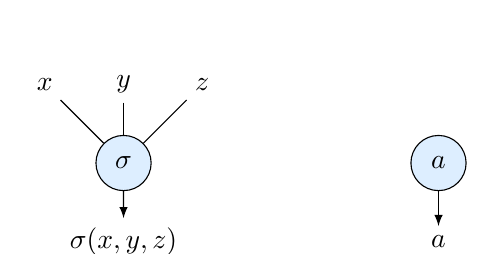
\begin{tikzpicture}
\draw (-1, 2) node(x1) {$x$} ;
\draw (0, 2) node(x2) {$y$} ;
\draw (1, 2) node(xr) {$z$} ;
  \draw (0, 1) \sdconstructor{sigma}{$\sigma$} ;
    \draw (0, 0) node(result) {$\sigma(x,y,z)$} ;
\draw[-latex] (x1) -- (sigma) -- (result) ;
\draw (x2) -- (sigma) ;
\draw (xr) -- (sigma) ;
\draw (4,1) \sdconstructor{a}{$a$} ;
  \draw (4,0) node(aresult) {$a$} ;
\draw[-latex] (a) -- (aresult) ;
\end{tikzpicture}
\end{center}

Thus the rules $0 = (~ \mid 0)$ and $s = (n \mid n+1)$ that describe the natural numbers can be expressed as follows:
\begin{center}
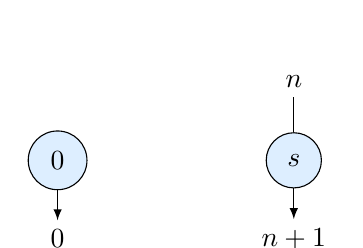
\begin{tikzpicture}
\draw (0,1) \sdconstructor{c0}{$0$} ;
  \draw (0,0) node(n0) {$0$} ;
\draw (3,2) node(varn) {$n$} ;
  \draw (3,1) \sdconstructor{s}{$s$} ;
    \draw (3,0) node(varsn) {$n+1$} ;
\draw[-latex] (c0) -- (n0) ;
\draw[-latex] (varn) -- (s) -- (varsn) ;
\end{tikzpicture}
\end{center}

These diagrams can be pieced together to represent the result of applying a rule to the outputs of other rules. For example:
\begin{center}
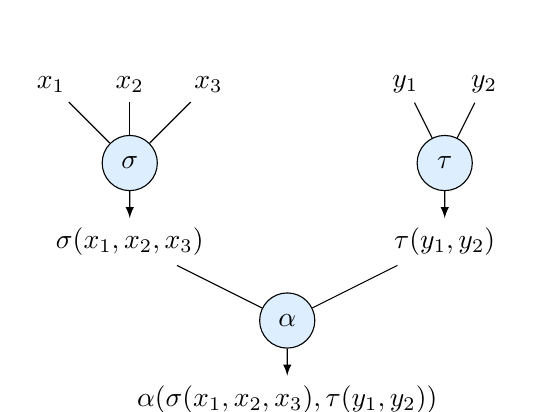
\begin{tikzpicture}
\draw (-3,4) node(a) {$x_1$} ;
\draw (-2,4) node(b) {$x_2$} ;
\draw (-1,4) node(c) {$x_3$} ;
  \draw (-2,3) \sdconstructor{sigma}{$\sigma$} ;
    \draw (-2,2) node(sigmares) {$\sigma(x_1,x_2,x_3)$} ;
\draw (1.5,4) node(x) {$y_1$} ;
\draw (2.5,4) node(y) {$y_2$} ;
  \draw (2,3) \sdconstructor{tau}{$\tau$} ;
    \draw (2,2) node(taures) {$\tau(y_1,y_2)$} ;
      \draw (0,1) \sdconstructor{alpha}{$\alpha$} ;
        \draw (0,0) node(alphares) {$\alpha(\sigma(x_1,x_2,x_3), \tau(y_1,y_2))$} ;
\draw[-latex] (a) -- (sigma) -- (sigmares) ;
\draw (b) -- (sigma) ;
\draw (c) -- (sigma) ;
\draw[-latex] (x) -- (tau) -- (taures) ;
\draw (y) -- (tau) ;
\draw[-latex] (sigmares) -- (alpha) -- (alphares) ;
\draw (taures) -- (alpha) ;
\end{tikzpicture}
\end{center}

This can be useful for seeing how an element of a set is obtained by applying the rules. For example, the following diagram shows how the natural number $3$ is obtained by applying the rules $(~ \mid 0)$ and $(n \mid n+1)$

\begin{center}
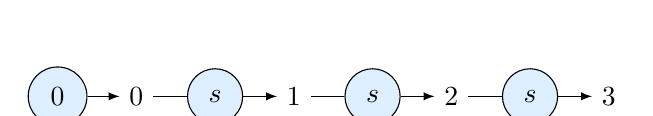
\begin{tikzpicture}
\draw (0,0) \sdconstructor{c0}{$0$} ;
  \draw (1,0) node(n0) {$0$} ;
    \draw (2,0) \sdconstructor{s1}{$s$} ;
      \draw (3,0) node(n1) {$1$} ;
        \draw (4,0) \sdconstructor{s2}{$s$} ;
          \draw (5,0) node(n2) {$2$} ;
            \draw (6,0) \sdconstructor{s3}{$s$} ;
              \draw (7,0) node(n3) {$3$} ;
\draw[-latex] (c0) -- (n0) ;
\draw[-latex] (n0) -- (s1) -- (n1);
\draw[-latex] (n1) -- (s2) -- (n2) ;
\draw[-latex] (n2) -- (s3) -- (n3) ;
\end{tikzpicture}
\end{center}

The following diagram shows how the logical formula $(p \Rightarrow q) \wedge (\neg r)$ is obtained by applying the rules described in \Cref{exRulesForInductiveDefinitionOfPropositionalFormulae}.

\begin{center}
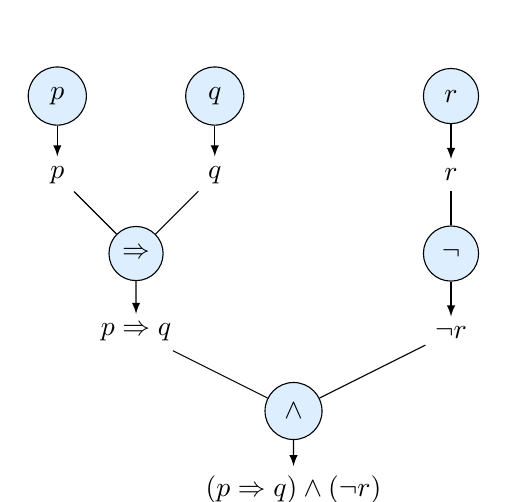
\begin{tikzpicture}
\draw (-3,5) \sdconstructor{cp}{$p$} ;
\draw (-1,5) \sdconstructor{cq}{$q$} ;
\draw (2,5) \sdconstructor{cr}{$r$} ;
\draw (-3,4) node(p) {$p$} ;
\draw (-1,4) node(q) {$q$} ;
  \draw (-2,3) \sdconstructor{implies}{$\Rightarrow$} ;
    \draw (-2,2) node(pimpliesq) {$p \Rightarrow q$} ;
\draw (2,4) node(r) {$r$} ;
  \draw (2,3) \sdconstructor{not}{$\neg$} ;
    \draw (2,2) node(notr) {$\neg r$} ;
      \draw (0,1) \sdconstructor{and}{$\wedge$} ;
        \draw (0,0) node(result) {$(p \Rightarrow q) \wedge (\neg r)$} ;
\draw[-latex] (cp) -- (p) ;
\draw[-latex] (cq) -- (q) ;
\draw[-latex] (cr) -- (r) ;
\draw[-latex] (p) -- (implies) -- (pimpliesq) ;
        \draw (q) -- (implies) ;
\draw[-latex] (r) -- (not) -- (notr) ;
\draw[-latex] (pimpliesq) -- (and) -- (result) ;
        \draw (notr) -- (and) ;
\end{tikzpicture}
\end{center}

\begin{exercise}
Let $\Sigma = \{ a,b,c,d \}$. Draw a diagram to represent how the word $cbadbd \in \Sigma^*$ can be obtained by applying the rules you defined in \Cref{exRulesForInductiveDefinitionOfWords}.
\end{exercise}

We are now ready to define an inductively defined set.

\begin{definition}
\label{defInductivelyDefinedSet}
\index{inductively defined set}
\index{set!inductively defined}
\index{constructor}
An \textbf{inductively defined set} is a set $A$ equipped with a set $R$ of rules and, for each rule $\sigma = (\mathbf{x} \mid \sigma(\mathbf{x})) \in R$, a function $f_{\sigma} : A^{\mathrm{ar}(\sigma)} \to A$, such that:
\begin{enumerate}[(a)]
\item For each $a \in A$, there is a unique rule $\sigma \in R$ and a unique $\mathrm{ar}(\sigma)$-tuple $\mathbf{a} = (a_0,a_1,\dots,a_{\mathrm{ar}(\sigma)-1}) \in A^{\mathrm{ar}(\sigma)}$ such that $a = f_{\sigma}(\mathbf{a})$; and
\item For all $B \subseteq A$, if $f_{\sigma}(\mathbf{a}) \in B$ for all $\sigma \in R$ and all $\mathbf{a} \in B^{\mathrm{ar}(\sigma)}$, then $B = A$.
\end{enumerate}
Given a rule $\sigma$, the function $f_{\sigma} : A^{\mathrm{ar}(\sigma)} \to A$ is called the \textbf{constructor} associated with $\sigma$; we may at times refer to the \textbf{arity} of the constructor $f_{\sigma}$ to mean the arity of the associated rule $\sigma$.
\end{definition}

Note that nullary constructors are the same thing as elements of $A$. Indeed, $A^0 = \{ () \}$, where $()$ is the empty list of elements of $A$, and so specifying a function $f_{\sigma} : A^0 \to A$ is equivalent to specifying an element $f_{\sigma}(\,()\,) \in A$. In this sense, we may regard nullary constructors as \textit{being} the elements of $A$---we call such elements \textit{basic elements}.

\begin{definition}
\label{defBasicElement}
\index{basic element}
\index{element!basic}
A \textbf{basic element} of an inductively defined set $A$ is an element of $A$ that is the value of a nullary constructor $f_{\sigma} : A^0 \to A$. If $\sigma = (~ \mid a)$ is a nullary rule, we will denote this element by $a$---thus we have $a = f_{\sigma}(\,()\,) \in A$ for all nullary rules $\sigma = (~ \mid a)$.
\end{definition}

Considering basic elements separately from constructors of positive arity has its pros and cons, so we will take whichever approach is most convenient for us at any given point in time. Unless otherwise specified, we will not separate nullary constructors from the others.

We have already seen some examples of inductively defined sets---let's prove that they truly \textit{are} inductively defined sets!

\begin{proposition}
\label{propNIsInductivelyDefined}
The set $\mathbb{N}$ of natural numbers is inductively defined by the rules $(~ \mid 0)$ and $(n \mid n+1)$.
\end{proposition}

\begin{cproof}
Since $(~ \mid 0)$ is a nullary rule, it will correspond to a basic element of $\mathbb{N}$---it may be no surprise that we take this element to be the natural number $0$.

The rule $s = (n \mid n+1)$ induces a function $f_s : \mathbb{N} \to \mathbb{N}$; we take this to be the successor function, defined by $f_s(n) = n+1$ for all $n \in \mathbb{N}$.

Now we must verify conditions (a) and (b) of \Cref{defInductivelyDefinedSet}.
\begin{enumerate}[(a)]
\item Let $n \in \mathbb{N}$.
\begin{itemize}
\item If $n = 0$, then since $0$ is a basic element and $0 \ne n+1 = f_s(n)$ for any $n \in \mathbb{N}$, we have that `$0$' is the unique expression of $0$ as a (nullary) constructor applied to (no) elements of $\mathbb{N}$.
\item If $n > 0$, then $n-1 \in \mathbb{N}$ and $n = (n-1)+1 = f_s(n-1)$. Moreover if $m \in \mathbb{N}$ and $n=f_s(m)$, then $n=m+1$, so that $m=n-1$. Moreover $n \ne 0$, meaning that there is a unique rule (namely $s$) and a unique natural number $m$ (namely $m=n-1$) such that $n=f_s(m)$.
\end{itemize}
\item Let $X$ be a set, and assume that $0 \in X$ and $f_s(n) \in X$ for all $n \in \mathbb{N}$. Then condition (iii) of \Cref{defNotionOfNaturalNumbers} ensures that $\mathbb{N} \subseteq X$.
\end{enumerate}

Thus $\mathbb{N}$ is inductively defined by $(~ \mid 0)$ and $(n \mid n+1)$, as required.
\end{cproof}

\begin{example}
\label{exInductivelyDefinedSetOfPropositionalFormulae}
Let $P$ be a set of propositional variables. In order to exhibit $\mathcal{L}(P)$ as an inductively defined set, we should be slightly more precise about the role of \textit{\gbus{brackets}{parentheses}} in propositional formulae than we have been so far.

For example, if we take the rules discussed in \Cref{exPropositionalFormulaeAsInductivelyDefinedSetPreliminary} literally, then $p \wedge q \vee r$ would be a valid logical formula. This is problematic for two reasons: first, does it mean $(p \wedge q) \vee r$, or $p \wedge (q \vee r)$? These are not logically equivalent, so the distinction matters. Second, this causes the `uniqueness' part of \Cref{defInductivelyDefinedSet} to fail, since $p \wedge q \vee r = f_{\wedge}(p,f_{\vee}(q,r)) = f_{\vee}(f_{\wedge}(p,q),r)$.

To remedy this, we will require parentheses to be added whenever we introduce a logical operator. Thus the rules defining a logical formula are:
\[ \underbrace{(~ \mid p)}_{\text{one for each } p \in P} \quad (\varphi,\psi \mid (\varphi \wedge \psi)\,) \quad (\varphi,\psi \mid (\varphi \vee \psi)\,) \quad (\varphi,\psi \mid (\varphi \Rightarrow \psi)\,) \quad (\varphi \mid (\neg \varphi)\,) \]

Thus $p \wedge q \vee r$ is not a valid element of $\mathcal{L}(P)$, but $((p \wedge q) \vee r)$ and $(p \wedge (q \vee r))$ are.
\end{example}

\begin{exercise}
Let $\Sigma$ be an alphabet. Prove that $\Sigma^*$ is inductively defined by the rules $(~ \mid \varepsilon)$ and $\sigma_a = (w \mid wa)$ for $a \in \Sigma$.
\end{exercise}

\begin{exercise}
Prove that $\mathbb{N}$ is inductively defined by the rules $(~ \mid 0)$, $(~ \mid 1)$ and $(n \mid n+2)$.
\end{exercise}

\subsection*{Defining new inductively defined sets}

Now that we have seen what it means for an \textit{already defined} set to be inductively defined, it would be useful to be able to \textit{make definitions} of inductively defined sets. Based on what we have seen so far, in order to define an inductively defined set, all we should need to do is specify a set of rules that tell us how to generate its elements.

We now prove that it really is that simple!

\begin{definition}
\label{defSetGeneratedByRules}
Let $R$ be a set of rules. The set \textbf{generated by} $R$ is defined by $A = \bigcup_{n \in \mathbb{N}} A_n$, where the sets $A_n$ for $n \in \mathbb{N}$ are defined recursively by:
\begin{itemize}
\item $A_0 = \left\{ a \middlemid (~\mid a) \in R \right\}$; and
\item $A_{n+1} = \left\{ \sigma(\mathbf{a}) \middlemid \mathbf{a} \in A_n^{\mathrm{ar}(\sigma)},~ (\mathbf{x} \mid \sigma(\mathbf{x})) \in R \right\}$.
\end{itemize}
That is, $A_0$ is the set of symbols to the right of the bar `$\mid$' in the nullary rules in $R$, and $A_{n+1}$ is the set of all expressions obtained by substituting the elements of $A_n$ symbol-by-symbol for the variables in the expressions to the right of the bar the other rules.
\end{definition}

\begin{example}
Let $N$ be the set generated by the rules $(~ \mid z)$ and $(n \mid s(n))$. Then
\begin{itemize}
\item $N_0 = \{ z \}$, since $(~ \mid z)$ is the only nullary rule.
\item $N_1$ is the result of applying the rules to the elements of $N_0$, of which there is only one, namely $z$. Applying the rule $(~\mid z)$ (to no elements, since it is nullary) gives $z$; applying the rule $(n \mid s(n))$ to $z$ gives $s(z)$. So $N_1 = \{ z, s(z) \}$.
\item Continuing, we get $N_2 = \{ z, s(z), s(s(z)) \}$, and so on.
\end{itemize}
We thus have
\[ N ~=~ \bigcup_{n \in \mathbb{N}} N_n ~=~ \{ z, s(z), s(s(z)), s(s(s(z))), \dots \} \]
This looks an awful lot like the set of all natural numbers; and indeed it is, provided we interpret $z=0$ and $s(n)=n+1$ (like we did in \Cref{secPeanosAxioms}).
\end{example}

\begin{example}
\label{exParenthesisations}
Let $A$ be the set generated by the rules $(~ \mid \star)$ and $(x,y \mid [x,y])$. Then
\begin{itemize}
\item $A_0 = \{ \star \}$;
\item $A_1 = \{ \star,~ [\star, \star] \}$;
\item $A_2 = \{ \star,~ [\star, \star],~ [\star, [\star,\star]],~ [[\star, \star], \star],~ [[\star,\star],[\star,\star]] \}$;
\item \dots{} and so on.
\end{itemize}
Thus for each $n \in \mathbb{N}$, the set $A_n$ consists of all parenthesised lists of `$\star$'s, where the list has length between $1$ and $2^n$ (inclusive). This can be proved by induction on $n$.

Hence $A = \bigcup_{n \in \mathbb{N}} A_n$ is the set of all (finite) such lists.
\end{example}

\begin{exercise}
Let $R$ be a set of rules for an inductive definition and let $A$ be the set generated by $R$. Prove that if $R$ has no nullary rules, then $A$ is empty.
\end{exercise}

\begin{exercise}
Let $R$ be a set of rules for an inductive definition, and let $A$ be the set generated by $R$. Prove that if $R$ is countable, then $A$ is countable.
\end{exercise}

\begin{exercise}
\label{exSetGeneratedByRulesIsInductivelyDefined}
Let $R$ be a set of rules. Prove that the set $A$ generated by $R$ is inductively defined; for each rule $\sigma = (\mathbf{x} \mid \sigma(\mathbf{x}))$, the constructor $f_{\sigma} : A^{\mathrm{ar}(\sigma)} \to A$ is defined by
\[ f_{\sigma}(\mathbf{a}) ~=~ \sigma(\mathbf{a}) \]
where $\sigma(\mathbf{a})$ denotes the result of substituting the specific elements of $A$ listed in $\mathbf{a}$ for the respective variables listed in $\mathbf{x}$. [For example, if $\sigma = (x,y \mid [x \odot y])$ and $\mathbf{a} = (2,5)$, then $\sigma(2,5) = [2 \odot 5]$.]
\end{exercise}

\subsection*{Structural recursion}

The recursion theorem for the natural numbers (\Cref{thmRecursion}) says that we can define a function $h : \mathbb{N} \to X$ by specifying the value of $h(0)$, and for each $n \in \mathbb{N}$, specifying the value of $h(n+1)$ in terms of the value of $h(n)$. This makes intuitive sense: since every natural number is obtained from $0$ by adding one some finite number of times, if we know the value of $h(0)$, and we know how the value of $h$ changes when we add one to its argument, then we should know the value of $h(n)$ for all natural numbers $n$.

It turns out that there is nothing special about $\mathbb{N}$ here: exactly the same argument demonstrates that for \textit{any} inductively defined set $A$, if we know what a function $h : A \to X$ does to its basic elements, and we know how its values change when we apply a constructor to its arguments, then we should know the value of $h(a)$ for all $a \in A$.

The proof of the structural recursion theorem is one of the times where treating basic elements ($\equiv$ nullary constructors) separately from constructors of positive arity makes the proof more difficult; so we will phrase it entirely in terms of constructors.

\begin{theorem}[Structural recursion theorem]
\label{thmStructuralRecursion}
Let $A$ be an inductively defined set, let $X$ be a set, and for each rule $\sigma$, let
\[ h_{\sigma} : A^{\mathrm{ar}(\sigma)} \times X^{\mathrm{ar}(\sigma)} \to X \]
Then there is a unique function $h : A \to X$ such that
\[ h(f_{\sigma}(\mathbf{a})) ~=~ h_{\sigma}(\mathbf{a},h(\mathbf{a})) \]
for all rules $\sigma$ and all $\mathbf{a} \in A^{\mathrm{ar}(\sigma)}$, where $h(\mathbf{a}) = (h(a_1),\dots,h(a_{\mathrm{ar}(\sigma)}))$.
\end{theorem}

\begin{cproof}
Let $D = \{ a \in X \mid h(a) \text{ is defined} \} \subseteq A$. Let $\sigma$ be a rule let $\mathbf{a} \in D^{\mathrm{ar}(\sigma)}$. Define
\[ h(f_{\sigma}(\mathbf{a})) = h_{\sigma}(\mathbf{a},h(\mathbf{a})) \]
Note that this is defined, since the assumption that $\mathbf{a} \in D^{\mathrm{ar}(\sigma)}$ implies that $h(a_i)$ is defined for all $i \in [\mathrm{ar}(\sigma)]$. Therefore $f_{\sigma}(\mathbf{a}) \in D$.
By \Cref{defInductivelyDefinedSet}(b) we have $D=A$, so that $h(a)$ is defined for all $a \in A$, so that we have a function $h : A \to X$ as required.

To see that $h$ is unique, let $h' : A \to X$ and suppose that $h'$ satisfies the same equations as $h$, meaning that
\[ h'(f_{\sigma}(\mathbf{a})) = h_{\sigma}(\mathbf{a},h'(\mathbf{a})) \]
for all rules $\sigma$ and all $\mathbf{a} \in A^{\mathrm{ar}(\sigma)}$.

Let $E = \{ a \in A \mid h'(a) = h(a) \}$, let $\sigma$ be a rule, and let $\mathbf{a} \in E^{\mathrm{ar}(\sigma)}$. Then $h'(a_i) = h(a_i)$ for all $i \in [\mathrm{ar}(\sigma)]$, so that
\[ h'(f_{\sigma}(\mathbf{a})) = h_{\sigma}(\mathbf{a},h'(\mathbf{a})) = h_{\sigma}(\mathbf{a},h(\mathbf{a})) = h(f_{\sigma}(\mathbf{a})) \]
and hence $f_{\sigma}(\mathbf{a}) \in E$. By \Cref{defInductivelyDefinedSet}(b) again, we have $E = A$, so that $h'(a) = h(a)$ for all $a \in A$. Therefore $h'=h$ by function extensionality.
\end{cproof}

\begin{strategy}[Defining functions by structural recursion]
\label{strStructuralRecursion}
Let $A$ be an inductively defined set and let $X$ be a set. In order to specify a function $h : A \to X$, it suffices to define $h(a)$ for all basic elements $a \in A$, and for each rule $\sigma$, to define $h(f_{\sigma}(\mathbf{a}))$ in terms of the values of $h(a_i)$ for each $i \in [\mathrm{ar}(\sigma)]$.
\end{strategy}

\begin{example}
Let $\mathcal{L}(P)$ be the inductively defined set of propositional formulae over a set $P$ of propositional variables. Define $h : \mathcal{L}(P) \to \mathbb{N}$ recursively as follows:
\begin{enumerate}[(i)]
\item Let $h(p) = 0$ for all $p \in P$;
\item For all $\varphi, \psi \in \mathcal{L}(P)$, let $h(\varphi \wedge \psi) = h(\varphi) + h(\psi) + 1$;
\item For all $\varphi, \psi \in \mathcal{L}(P)$, let $h(\varphi \vee \psi) = h(\varphi) + h(\psi) + 1$;
\item For all $\varphi, \psi \in \mathcal{L}(P)$, let $h(\varphi \Rightarrow \psi) = h(\varphi) + h(\psi) + 1$;
\item For all $\varphi \in \mathcal{L}(P)$, let $h(\neg \varphi) = h(\varphi) + 1$.
\end{enumerate}
By the structural recursion theorem, this completely determines the function $h$.

For example
\begin{align*}
& h((p \Rightarrow q) \wedge (\neg r)) && \\
&= h(p \Rightarrow q) + h(\neg r) + 1 && \text{by (ii)} \\
&= [h(p) + h(q) + 1] + [h(r) + 1] + 1 && \text{by (iv) and (v)} \\
&= [0+0+1] + [0+1] + 1 && \text{by (i)} \\
&= 3
\end{align*}

More generally, for each $\varphi \in \mathcal{L}(P)$, the value $h(\varphi)$ is the number of logical operators that appear in $\varphi$. We can prove this by \textit{structural induction}---more on this soon.
\end{example}

\begin{definition}
\label{defRank}
\index{rank}
\nindex{rk}{$\mathrm{rk}(a)$}{rank}
Let $A$ be an inductively defined set. The \textbf{rank} $\mathrm{rk}(a)$ \inlatex{mathrm\{rk\}}\lindexmmc{mathrm}{$\mathrm{Aa}, \mathrm{Bb}, \dots$} of an element $a \in A$ is defined by recursively by letting $\mathrm{rk}(a) = 0$ for all basic elements $a$, and
\[ \mathrm{rk}(f_{\sigma}(\mathbf{a})) = \mathrm{max} \{ \mathrm{rk}(a_i) \mid i \in [\mathrm{ar}(\sigma)] \} + 1 \]
for all rules $\sigma$ and all $\mathbf{a} \in A^{\mathrm{ar}(\sigma)}$.
\end{definition}

Intuitively, the rank of an element $a \in A$ tells us how many `layers' of constructors (of positive arity) appear in the unique expression of $a$ as constructors applied to basic elements.

\begin{example}
Let $P$ be a set of propositional variables, let $p,q,r,s \in P$, and define
\[ \varphi = ((p \wedge q) \vee (r \Rightarrow (\neg s))) \in \mathcal{L}(P) \]
Intuitively, $s$ is the innermost propositional variable in $\varphi$, because in order to access $s$ we must first go through $\vee$, and then $\Rightarrow$, and then $\neg$; therefore we have three layers of constructors, so we expect to have $\mathrm{rk}(\varphi) = 3$. We will verify that we are correct.

Since $p,q,r,s \in P$ are basic elements of $\mathcal{L}(P)$, we have
\[ \mathrm{rk}(p)=\mathrm{rk}(q)=\mathrm{rk}(r)=\mathrm{rk}(s)=0 \]
Now we can iteratively find the ranks of the subformulae of $\varphi$:
\begin{itemize}
\item $\mathrm{rk}((p \wedge q)) = \mathrm{max} \{ 0, 0 \} + 1 = 0 + 1 = 1$;
\item $\mathrm{rk}((\neg s)) = \mathrm{max}\{ \mathrm{rk}(s) \} + 1 = \mathrm{max} \{ 0 \} + 1 = 0 + 1 = 1$;
\item $\mathrm{rk}(r \Rightarrow (\neg s)) = \mathrm{max} \{ \mathrm{rk}(r), \mathrm{rk}((\neg s)) \} + 1 = \mathrm{max} \{ 0, 1 \} + 1 = 1 + 1 = 2$;
\end{itemize}
and so finally we have
\[ \mathrm{rk}(\varphi) = \mathrm{max} \{ \mathrm{rk}((p \wedge q), (r \Rightarrow (\neg s)) \} + 1 = \mathrm{max} \{ 1, 2 \} + 1 = 2 + 1 = 3 \]
as expected.
\end{example}

\begin{example}
The rank of a natural number $n$ is $n$. Indeed we have $\mathrm{rk}(0) = 0$ since $0$ is a basic element, and for all $n \in \mathbb{N}$ we have $\mathrm{rk}(n+1) = \mathrm{max} \{ \mathrm{rk}(n) \} + 1 = \mathrm{rk}(n) + 1$. By the recursion theorem (take your pick from \Cref{thmRecursion} or \Cref{thmStructuralRecursion}), we have $\mathrm{rk}(n) = n$ for all $n \in \mathbb{N}$.
\end{example}

\begin{exercise}
Let $\Sigma$ be an alphabet and let $\Sigma^*$ be the inductively defined set of words over $\Sigma$. Prove that for all $w \in \Sigma$, the rank $\mathrm{rk}(w)$ is equal to the length of $W$. [We regard the empty string $\varepsilon$ to have length $0$, despite the fact that the placeholder character $\varepsilon$ is used to denote it.]
\end{exercise}

\subsection*{Structural induction}

We now derive the structural induction principle, which is used for proving that a property $p(x)$ is true for all elements $x$ of an inductively defined set $A$.

The idea behind structural induction is the same as the idea behind weak induction: since every element $a \in A$ is of the form $f_{\sigma}(\mathbf{a})$ for some (possibly nullary) rule $\sigma$, if we can prove that the truth of $p$ is preserved by applying each constructor $f_{\sigma}$, then $p(x)$ must be true for all $x \in A$. [In the case of nullary constructors, this amounts to checking that $p(a)$ is true for each basic element $a \in A$.]

Thus in order to prove $\forall x \in A,~ p(x)$, we need to prove that for every rule $\sigma$\dots{}

\begin{center}
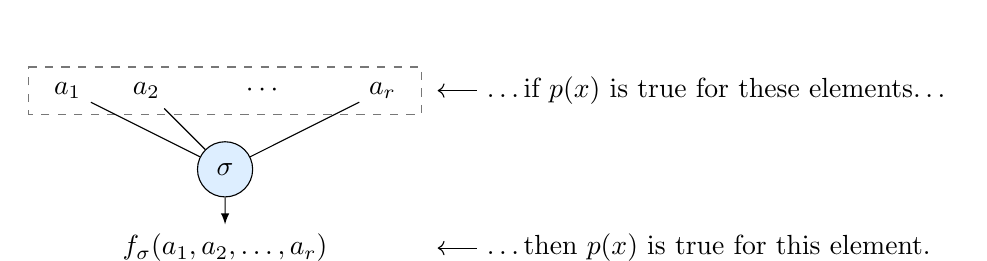
\begin{tikzpicture}
\draw (-2, 2) node(x1) {$a_1$} ;
\draw (-1, 2) node(x2) {$a_2$} ;
\draw (0.5, 2) node(dots) {$\cdots$} ;
\draw (2, 2) node(xr) {$a_r$} ;
  \draw (0, 1) \sdconstructor{sigma}{$\sigma$} ;
    \draw (0, 0) node(result) {$f_{\sigma}(a_1,a_2,\dots,a_r)$} ;
\draw[<-] (2.7, 2) -- (3.2,2) node[right] {\dots{}if $p(x)$ is true for these elements\dots{}} ;
\draw[<-] (2.7, 0) -- (3.2,0) node[right] {\dots{}then $p(x)$ is true for this element.} ;
\draw[midgray, dashed] (-2.5,2.3) -- (2.5,2.3) -- (2.5,1.7) -- (-2.5,1.7) -- cycle ;
\draw[-latex] (x1) -- (sigma) -- (result) ;
\draw (x2) -- (sigma) ;
\draw (xr) -- (sigma) ;
\end{tikzpicture}
\end{center}

Let's prove that this intuition is valid.

\begin{theorem}[Structural induction principle]
\label{thmStructuralInduction}
\index{induction!structural}
Let $A$ be an inductively defined set and let $p(x)$ be a logical formula with free variable $x \in A$. If for all rules $\sigma$ and all $\mathbf{a} \in A^{\mathrm{ar}(\sigma)}$ we have
\[ [\forall i \in [\mathrm{ar}(\sigma)],~ p(a_i)] \Rightarrow p(f_{\sigma}(\mathbf{a})) \]
then $p(x)$ is true for all $x \in A$.
\end{theorem}

\begin{cproof}
Assume that for all rules $\sigma$ and all $\mathbf{a} \in A^{\mathrm{ar}(\sigma)}$ we have
\[ [\forall i \in [\mathrm{ar}(\sigma)],~ p(a_i)] \Rightarrow p(f_{\sigma}(\mathbf{a})) \]

Let $X = \{ a \in A \mid p(a) \} \subseteq A$. Then for all $a \in A$ we have $a \in X$ if and only if $p(a)$ is true. Thus we have
\[ [\forall i \in [\mathrm{ar}(\sigma)],~ a_i \in X] \Rightarrow f_{\sigma}(\mathbf{a}) \in X \]
But this is exactly the hypothesis of condition (b) of \Cref{defInductivelyDefinedSet}, and so $A \subseteq X$.

Hence $A = X$, so that $p(a)$ is true for all $a \in A$, as required.
\end{cproof}

Let's digest the statement of \Cref{thmStructuralInduction}.

For a nullary rule $\sigma = (~ \mid a)$, the arity $\mathrm{ar}(\sigma)$ is $0$, so $\forall i \in [\mathrm{ar}(\sigma)],~p(a_i)$ is equivalent to $\forall i \in \varnothing,~ p(a_i)$, which is vacuously true (see \Cref{exEverythingIsTrueOfElementsOfEmptySet}), so that
\[ [\forall i \in [\mathrm{ar}(\sigma)],~ p(a_i)] \Rightarrow p(f_{\sigma}(\mathbf{a})) \quad \equiv \quad p(a) \]

Therefore, saying that $[\forall i \in [\mathrm{ar}(\sigma)],~ p(a_i)] \Rightarrow p(f_{\sigma}(\mathbf{a}))$ is true for all rules $\sigma$ and all $\mathbf{a} \in A^{\mathrm{ar}(\sigma)}$ is equivalent to saying:
\begin{itemize}
\item $p(a)$ is true for all basic elements $a$; and
\item $[\forall i \in [\mathrm{ar}(\sigma)],~ p(a_i)] \Rightarrow p(f_{\sigma}(\mathbf{a}))$ is true for all rules $\sigma$ of \textit{positive} arity and all $\mathbf{a} \in A^{\mathrm{ar}(\sigma)}$.
\end{itemize}

This suggests the following proof strategy.

\begin{strategy}[Proof by structural induction]
\index{proof!by structural induction}
\index{induction!on an inductively defined set}
In order to prove a proposition of the form $\forall a \in A,~ p(a)$, where $A$ is an inductively defined set, it suffices to prove for all rules $\sigma$ that
\[ [\forall i \in [\mathrm{ar}(\sigma)],~ p(a_i)] \Rightarrow p(f_{\sigma}(\mathbf{a})) \]
Equivalently, it suffices to:
\begin{itemize}
\item For each basic element $a \in A$, prove $p(a)$---this is the \textbf{base case} for $a$;
\item For each constructor $\sigma$ of arity $r>0$, let $a_1,a_2,\dots,a_r \in A$ and assume that $p(a_i)$ is true for all $i \in [r]$, and prove that $p(f_{\sigma}(a_1,a_2,\dots,a_r))$ is true---this is the \textbf{induction step} for $\sigma$.
\end{itemize}
The assumption $\forall i \in [r],~p(a_i)$ in the induction step for $\sigma$ is called the \textbf{induction hypothesis} for $\sigma$.
\end{strategy}

\begin{example}
The structural induction principle for the inductively defined set $\mathbb{N}$ is exactly the same as the weak induction principle (\Cref{thmWeakInduction}). It says that to prove $\forall n \in \mathbb{N},~ p(n)$ is true, it suffices to:
\begin{itemize}
\item Prove $p(0)$ is true (since $0$ is the only basic element); and
\item Let $n \in \mathbb{N}$, assume that $p(n)$ is true, and prove that $p(n+1)$ is true (since the successor operation is the only constructor of positive arity).
\end{itemize}
Thus we recover weak induction as a special case of structural induction.
\end{example}

\begin{example}
Fix a set $P$ of propositional variables and let $\mathcal{L}(P)$ be the inductively defined set of (properly \gbus{bracketed}{parenthesised}) propositional formulae over $P$, as in \Cref{exInductivelyDefinedSetOfPropositionalFormulae}.

We prove that every propositional formula $\varphi \in \mathcal{L}(P)$ has the same number of open \gbus{brackets}{parentheses} `$($' as closed \gbus{brackets}{parentheses} `$)$'.

\begin{itemize}
\item (\textbf{Base cases}) The basic elements of $\mathcal{L}(P)$ are the propositional variables $p \in P$. So let $p \in P$; this is a logical formula with no open \gbus{brackets}{parentheses} and no closed \gbus{brackets}{parentheses}, so the number of open \gbus{brackets}{parentheses} is equal to the number of closed \gbus{brackets}{parentheses}.

\item (\textbf{Induction step} for $\wedge$) Let $\varphi, \psi \in \mathcal{L}(P)$ and assume that $\varphi$ and $\psi$ each have the same number of open \gbus{brackets}{parentheses} as closed \gbus{brackets}{parentheses}. Say $\varphi$ has $a$ open \gbus{brackets}{parentheses} and $a$ closed \gbus{brackets}{parentheses}, and $\psi$ has $b$ open \gbus{brackets}{parentheses} and $b$ closed \gbus{brackets}{parentheses}, where $a,b \in \mathbb{N}$. Now
\[ f_{\wedge}(\varphi, \psi) ~=~ (\varphi \wedge \psi) \]
Since $\varphi$ contributes $a$ open \gbus{brackets}{parentheses} and $\psi$ contributes $b$ open \gbus{brackets}{parentheses}, this has $a+b+1$ open \gbus{brackets}{parentheses}; likewise it has $a+b+1$ closed \gbus{brackets}{parentheses}.

This completes the induction step for $\wedge$.

\item (\textbf{Induction steps} for $\vee$ and $\Rightarrow$) These are identical to the induction step for $\wedge$---just replace $\wedge$ by the necessary logical operator throughout.

\item (\textbf{Induction step} for $\neg$) Let $\varphi \in \mathcal{L}(P)$ and assume that $\varphi$ has the same number of open \gbus{brackets}{parentheses} as closed \gbus{brackets}{parentheses}---say it has $a$ of each, where $a \in \mathbb{N}$. Then
\[ f_{\neg}(\varphi) ~=~ (\neg \varphi) \]
Since $\varphi$ contributes $a$ open \gbus{brackets}{parentheses}, this has $a+1$ open \gbus{brackets}{parentheses}; likewise it has $a+1$ closed \gbus{brackets}{parentheses}.

This completes the induction step for $\neg$.
\end{itemize}

So by structural induction, it follows that every propositional formula $\varphi \in \mathcal{L}(P)$ has the same number of open \gbus{brackets}{parentheses} as closed \gbus{brackets}{parentheses}.
\end{example}

\begin{exercise}
Let $P$ be a set of propositional variables. Prove by structural induction that the rank of a propositional formula $\varphi \in \mathcal{L}(P)$ is equal to the number of logical operators in $\varphi$.
\end{exercise}

A nice application of structural induction is to provide a formula for the \textit{totient} of an integer $n$ (\Cref{defTotient}). We proved such a formula in \Cref{secModularArithmetic}, but that proof relied on the heavy machinery of the Chinese remainder theorem (\Cref{thmChineseRemainder})---here we give a proof without it.

\rthmTotientFormula*

\begin{cproof}
%% BEGIN EXTRACT (xtrWlogExample) %%
Recall that $\varphi(-n) = \varphi(n)$ for all $n \in \mathbb{Z}$, so we may assume without loss of generality that $n \ge 0$---otherwise just replace $n$ by $-n$ throughout.
%% END EXTRACT %%
Moreover
\[ \varphi(0) ~=~ 0 ~=~ 0 \cdot \prod_{p \mid n} \left( 1- \frac{1}{p} \right) \]
so for the rest of the proof, assume that $n>0$.

Let $P$ be the set of all positive prime numbers, and let
\[ A ~=~ \bigcup_{n \in \mathbb{N}} P^n ~=~ \{ (p_1,p_2,\dots,p_k) \mid k \in \mathbb{N},~ p_1,p_2,\dots,p_k \in P \} \]
The elements of $A$ are precisely lists of positive primes of finite length. Note that $A$ is inductively defined by the rules
\[ (~ \mid ()\,) \quad \text{and} \quad \sigma_q = (x \mid (x,q)) \text{ for each } q \in P \]
That is, the empty list $()$ is an element of $A$, and for each $(p_1,p_2,\dots,p_k) \in A$ and $q \in P$, we have $(p_1,p_2,\dots,p_k,q) \in A$.

By the fundamental theorem of arithmetic (\Cref{thmFTA}) there is a surjection $\Pi : A \to \{ n \in \mathbb{Z} \mid n > 0 \}$ defined by
\[ \Pi(p_1,p_2,\dots,p_k) ~=~ \prod_{i=1}^k p_i ~=~ p_1 \times p_2 \times \cdots \times p_k \]
for all $k \in \mathbb{N}$ and $p_1,p_2,\dots,p_k \in P$. Note in particular that $\Pi(\,()\,) = 1$, where $()$ is the empty list.

We prove by structural induction on $(p_1,p_2,\dots,p_k) \in A$ that the integer $n = \Pi(p_1,p_2,\dots,p_k) > 0$ satisfies the formula in the statement of the theorem. 

\begin{itemize}
\item (\textbf{Base case}) The unique basic element of $A$ is the empty list $()$. Since $\Pi(\,()\,) = 1$, we must prove that the equation in the statement of the theorem is satisfied when $n=1$. Well there are no primes $p$ such that $p \mid 1$, and so the product $\prod_{p \mid 1} \left( 1 - \frac{1}{p} \right)$ is the empty product, which is equal to $1$. Thus
\[ \varphi(1) ~=~ 1 ~=~ 1 \cdot 1 ~=~ 1 \cdot \prod_{p \mid 1} \left( 1- \frac{1}{p} \right) \]
as required.

\item (\textbf{Induction step} for $q \in P$) Fix $(p_1,p_2,\dots,p_k) \in A$, let $n = \Pi(p_1,p_2,\dots,p_k)$ and assume that
\[ \varphi(n) ~=~ n \cdot \prod_{p \mid n} \left( 1 - \frac{1}{p} \right) \]
Note that $\Pi(p_1,p_2,\dots,p_k,q) = qn$, and so we need to prove that
\[ \varphi(qn) ~=~ qn \cdot \prod_{p \mid qn} \left( 1 - \frac{1}{p} \right) \]
Now either $q \mid n$ or $q \nmid n$.
\begin{itemize}
\item Assume $q \mid n$. Then $n$ and $qn$ have the same prime divisors, and so for all $p \in P$ we have $p \mid n$ if and only if $p \mid qn$. Therefore:
\begin{align*}
\varphi(qn) &= q\varphi(n) && \text{by \Cref{exTotientMultiplyByPrime}} \\
&= qn \cdot \prod_{p \mid n} \left( 1-\frac{1}{p} \right) && \text{by induction hypothesis} \\
&= qn \cdot \prod_{p \mid qn} \left( 1-\frac{1}{p} \right) && \text{as observed above}
\end{align*}
as required.

\item Assume $q \nmid n$. Then for all $p \in P$ we have $p \mid qn$ if and only if $p \mid n$ or $p=q$. Therefore:
\begin{align*}
\varphi(qn) &= (q-1)\varphi(n) && \text{by \Cref{exTotientMultiplyByPrimeTwo}} \\
&= (q-1) n \cdot \prod_{p \mid n} \left( 1 - \frac{1}{p} \right) && \text{by induction hypothesis} \\
&= qn \left( 1 - \frac{1}{q} \right) \cdot \prod_{p \mid n} \left( 1 - \frac{1}{p} \right) && \text{rearranging} \\
&= qn \cdot \prod_{p \mid qn} \left( 1 - \frac{1}{p} \right) && \text{absorbing $1-\frac{1}{q}$ into the product}
\end{align*}

as required.
\end{itemize}

In both cases, the formula in the statement of the theorem is satisfied by the integer $qn$.
\end{itemize}

By structural induction, the result follows.
\end{cproof}

\subsection*{Uniqueness of inductive definitions}

It would be nice if an inductive definition completely characterises the set that it defines. But this is slightly too much to ask; for example, the sets
\[ \{ 0, 1, 2, 3, \dots \} \quad \text{and} \quad \{ \varepsilon, {\bullet}, {\bullet} {\bullet}, {\bullet} {\bullet} {\bullet}, \dots \} \]
are both inductively defined by the rules $(~ \mid z)$ and $(n \mid s(n))$. In the first we take the basic element $z$ to be the natural number $0$, and for each natural number $n$ we take $s(n)$ to be the natural number $n+1$; in the second, we take the basic element $z$ to be the empty word $\varepsilon$, and for each string $n$ we take $s(n)$ to be the string `$n {\bullet}$' (so for example $s({\bullet} {\bullet}) = {\bullet} {\bullet} {\bullet}$).

But there is evidently a way of translating between these sets: we can define a function from the first to the second by sending each natural number $n$ to the string ${\bullet} {\bullet} \cdots {\bullet}$, where there are $n$ `${\bullet}$'s in the string.

Thus the sets $\{ 0, 1, 2, 3, \dots \}$ and $\{ \varepsilon, {\bullet}, {\bullet}{\bullet}, {\bullet}{\bullet}{\bullet}, \dots \}$ are `essentially the same'---they are inductively defined by the same rules, and so the only real difference is how we \textit{label} their elements.

The next theorem demonstrates that the same is true of inductively defined sets in general. That is, if two sets $A$ and $B$ are inductively defined by the same rules, then the only way that they can differ is in the labels we use to denote their elements. Formally, this `relabelling' establishes a bijection $h : A \to B$ between the two sets.

In fact, we prove something stronger: not only is there a bijection between the two sets, but the bijection respects the constructors---that is, if we apply a constructor in $A$ to some elements and relabel the result, that is equivalent to relabelling the elements first and then applying the corresponding constructor in $B$. Even better, this bijection is the unique bijection that does so.

Thus to sum up what the following theorem tells us: inductively defined sets are \textit{uniquely} determined by their defining rules, up to a \textit{unique} bijection that is compatible with the constructors---this is as close to absolute uniqueness as we could possibly hope to get!

\begin{theorem}[Uniqueness of inductively defined sets]
\label{thmUniquenessOfInductivelyDefinedSets}
Let $A$ and $B$ be two sets that are inductively defined by the same set of rules. For each rule $\sigma$, let $f_{\sigma} : A^{\mathrm{ar}(\sigma)} \to A$ and $g_{\sigma} : B^{\mathrm{ar}(\sigma)} \to B$ be the respective constructors.

There is a unique bijection $h : A \to B$ such that
\[ h(f_{\sigma}(\mathbf{a})) ~=~ g_{\sigma}(h(\mathbf{a})) \]
where $h(\mathbf{a}) = (h(a_0), \dots, h(a_{\mathrm{ar}(\sigma) - 1}) \in B^{\mathrm{ar}(\sigma)}$.
\end{theorem}

\begin{cproof}
Define $h : A \to B$ by structural recursion as follows: given a rule $\sigma$ given $\mathbf{a} \in A^{\mathrm{ar}(\sigma)}$ such that $h(a_i)$ has been defined for all $i \in [\mathrm{ar}(\sigma)]$, define
\[ h(f_{\sigma}(\mathbf{a})) ~=~ g_{\sigma}(h(\mathbf{a})) \]
We just need to prove that $h$ is a bijection, since evidently the other condition on $h$ is satisfied by construction.

So define $k : B \to A$ by structural recursion on the same way; note that now we have
\[ k(g_{\sigma}(\mathbf{b})) ~=~ f_{\sigma}(k(\mathbf{b})) \]
where $k(\mathbf{b}) = (k(b_0),\dots,k(b_{\mathrm{ar}(\sigma)-1})) \in A^{\mathrm{ar}(\sigma)}$.

We prove that $k(h(a)) = a$ for all $a \in A$ by structural induction. To this end, let $\sigma$ be a rule, let $\mathbf{a} \in A^{\mathrm{ar}(\sigma)}$ and suppose that $k(h(a_i)) = a_i$ for all $i \in [\mathrm{ar}(\sigma)]$. Note that with the notation conventions we are using, this induction hypothesis can be more concisely stated as saying that $k(h(\mathbf{a})) = \mathbf{a}$.

Let $a = f_{\sigma}(\mathbf{a})$. Then
\begin{align*}
k(h(a))
&= k(h(f_{\sigma}(\mathbf{a}))) && \text{by definition of $a$} \\
&= k(g_{\sigma}(h(\mathbf{a}))) && \text{by construction} \\
&= f_{\sigma}(k(h(\mathbf{a})) && \text{by construction} \\
&= f_{\sigma}(\mathbf{a}) && \text{by induction hypothesis} \\
&= a && \text{by definition of $a$}
\end{align*}
This completes the induction step. So we have $k(h(a)) = a$ for all $a \in A$.

A similar proof by structural induction reveals that $h(k(b)) = b$ for all $b \in B$.

Thus $k$ is an inverse for $h$, so that $h$ is a bijection.

The fact that $h$ is the \textit{unique} such bijection is immediate from the fact that it is defined by structural recursion, with the recursive formula being equivalent to the assertion that $h$ respects constructors.
\end{cproof}

\begin{example}
Let $\Sigma$ be an alphabet. Then leaf-labelled rooted planar binary trees over $\Sigma$ are essentially the same as parenthesisations of lists of elements of $\Sigma$ of positive length.

Indeed, let $R$ be the set of rules defined by
\[ R = \{ (~ \mid a) \mid a \in \Sigma \} \cup \{ (t_1,t_2 \mid [t_1,t_2]) \} \]

Like in \Cref{exParenthesisations}, the inductively defined set $A$ generated by $R$ is given by the set of all parenthesisations of lists of elements of $\Sigma$. For example
\[ [[[a_1,a_2],a_3],[a_4,a_5]] \in A \]
where $a_1,a_2,a_3,a_4,a_5 \in \Sigma$.

But the set $T$ of all leaf-labelled rooted planar binary trees over $\Sigma$ is also inductively defined by the rules in $R$. The basic element $a$ corresponding to the rule $(~ \mid a)$ is precisely the tree consisting of just its root, which is labelled by the element $a \in \Sigma$:
\begin{center}
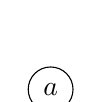
\begin{tikzpicture}
\draw (0,0) node[circle, draw] {$a$} ;
\end{tikzpicture}
\end{center}
and given trees $t_1,t_2$, the tree corresponding to $[t_1,t_2]$ is given by forming a tree with a root and two branches, pasting $t_1$ onto the left branch, and pasting $t_2$ onto the right branch:
\begin{center}
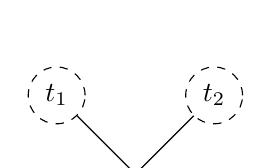
\begin{tikzpicture}
\draw (-1,1) node[circle, dashed, draw](t1) {$t_1$} ;
\draw (1,1) node[circle, dashed, draw](t2) {$t_2$} ;
  \draw[fill=black] (0,0) circle[radius=1.5pt] coordinate(root) ;
\draw (t1) -- (root) -- (t2) ;
\end{tikzpicture}
\end{center}

By \Cref{thmUniquenessOfInductivelyDefinedSets}, there is a unique bijection $A \to T$ that is compatible with the constructors in each set. For example, the element $[[[a_1,a_2],a_3],[a_4,a_5]] \in A$ corresponds with the following tree:
\begin{center}
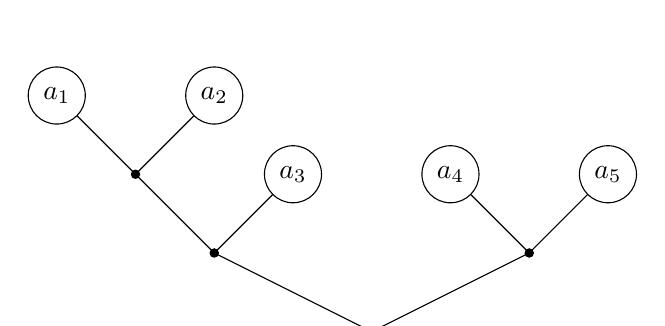
\begin{tikzpicture}
\draw[fill=black] (0,0) circle[radius=1.5pt] coordinate(root) ;
  \draw[fill=black] (-2,1) circle[radius=1.5pt] coordinate(rabc) ;
    \draw[fill=black] (-3,2) circle[radius=1.5pt] coordinate(rab) ;
      \draw (-4,3) node[circle, draw](a) {$a_1$} ;
      \draw (-2,3) node[circle, draw](b) {$a_2$} ;
    \draw (-1,2) node[circle, draw](c) {$a_3$} ;
  \draw[fill=black] (2,1) circle[radius=1.5pt] coordinate(rde) ;
    \draw (1,2) node[circle, draw](d) {$a_4$} ;
    \draw (3,2) node[circle, draw](e) {$a_5$} ;
\draw (root) -- (rabc) -- (rab) -- (a) ;
                    \draw (rab) -- (b) ;
          \draw (rabc) -- (c) ;
\draw (root) -- (rde) -- (d) ;
          \draw (rde) -- (e) ;
\end{tikzpicture}
\end{center}
\end{example}

\subsection*{\optmark{Quotient-inductive sets}}

Some sets appear to be inductively defined, in the sense that its elements can be constructed from some basic elements by applying some constructors, except there may be more than one way of expressing each of its elements as a constructor applied to some elements of the set.

For example, consider the set $\mathbb{Z}$ of integers. Every integer $n$ can be obtained from $0$ by either adding $1$ or subtracting $1$ some number of times. Thus we'd like to say that $\mathbb{Z}$ is inductively defined by the rules
\[ (~ \mid 0) \quad s = (x \mid x+1) \quad p = (x \mid x-1) \]
Here $s$ stands for `successor' and $p$ stands for `predecessor'. However, strictly 	speaking, $\mathbb{Z}$ is not inductively defined by these rules; for example
\[ 2 = 1 + 1 = f_s(1) \quad \text{and} \quad 2 = 3 - 1 = f_p(3) \]
and so $2$ does not have a \textit{unique} expression as a constructor applied to an integer.

In fact, the inductively defined set $A$ generated by the three rules above consists of all strings of the form
\[ 0 \pm 1 \pm 1 \pm \cdots \pm 1 \]
with each $\pm$ sign being either $+$ or $-$. We recover the corresponding integer by evaluating the string; this evaluation function defines a \textit{surjection} $q : A \to \mathbb{Z}$; for example
\[ q(0+1+1) = 2 \quad \text{and} \quad q(0+1+1+1-1+1-1-1+1) = 2 \]
As made precise in \Cref{thmEquivalenceRelationsSurjections}, the fact that there is a surjection $A \to \mathbb{Z}$ means that we can think of $\mathbb{Z}$ as being a quotient of $A$ by a suitable equivalence relation.

To see what this equivalence relation is, note that $(n+1)-1 = n$ and $(n-1)+1=n$ for all $n \in \mathbb{Z}$. Thus in a string $0 \pm 1 \pm \cdots \pm 1$, we can add or remove instances of `$+1-1$' or `$-1+1$' in the string as we please, and we will obtain the same integer. So define an equivalence relation $\sim$ on $A$ by letting $a \sim b$ if and only if the string $b$ can be obtained from $a$ by adding or removing `$+1-1$' or `$-1+1$' some number of times; for example
\[ 0+1+1 \quad \sim \quad 0+1-1+1+1 \quad \sim \quad 0+1+1+1-1+1-1-1+1 \]
Then $\sim$ is an equivalence relation on $A$, and the evaluation function $q : A \to \mathbb{Z}$ descends to a bijection $\bar q : A/{\sim} \to \mathbb{Z}$.

We will call sets obtained in this way \textit{quotient-inductive sets}.

\begin{definition}
\label{defFunctionRespectsRule}
Let $A$ be an inductively defined set and let $\sigma$ be a rule. A function $h : A \to X$ with domain $A$ \textbf{respects} $\sigma$ if, for all $\mathbf{a},\mathbf{b} \in A^{\mathrm{ar}(\sigma)}$, we have
\[ [\forall i \in [\mathrm{ar}(\sigma)],~ h(a_i) = h(b_i)] \quad \Rightarrow \quad h(f_{\sigma}(\mathbf{a})) = h(f_{\sigma}(\mathbf{b})) \]
\end{definition}

\todo{Example, exercise}

\begin{definition}
\label{defQuotientInductiveSet}
\index{set!quotient-inductive}
\index{quotient!quotient-inductive set}
\index{inductively defined set!quotient-inductive}
A \textbf{quotient-inductive set} is a set $Q$ equipped with a surjection $q : A \to Q$ for some inductively defined set $A$, such that $q$ respects all of the rules of $A$.

The function $q$ is called the \textbf{quotient map}; the \textbf{basic elements}, \textbf{constructors} and \textbf{rules} of $Q$ are the images under $q$ of those of $A$.
\end{definition}

We will abuse notation slightly in the following way. Given a rule $\sigma$ and $\mathbf{u} \in Q^{\mathrm{ar}(\sigma)}$, we will write $f_{\sigma}(\mathbf{u})$ instead of $q(f_{\sigma}(\mathbf{a}))$, where $\mathbf{a} \in A^{\mathrm{ar}(\sigma)}$ is such that $q(a_i) = u_i$ for each $i \in [\mathrm{ar}(\sigma)]$. Note that this is well-defined: the elements $a_i$ for $i \in [\mathrm{ar}(\sigma)]$ exist since $q$ is surjective, and the value of $q(f_{\sigma}(\mathbf{a}))$ is independent on the choices of $a_i$ picked since $q$ respects the rules of $A$.

\begin{example}
As we discussed, the rules $(~ \mid 0)$, $s = (x \mid x+1)$ and $p = (x \mid x-1)$ give rise to an inductively defined set $A$ whose elements are strings of the form $0 \pm 1 \pm 1 \pm \cdots \pm 1$, with each `$\pm$' sign replaced with either $+$ or $-$.

The function $q : A \to \mathbb{Z}$ given by evaluating the string is evidently a surjection: indeed, given $n \in \mathbb{Z}$, if $n \ge 0$ then $n = q(0+\underbrace{1+\cdots+1}_{\text{$n$ `$1$'s}})$, and if $n < 0$ then $n = q(0-\underbrace{1-\cdots-1}_{\text{$|n|$ `$1$'s}})$.

Thus $\mathbb{Z}$ is a quotient-inductive set, with basic element $0$ and constructors `$+1$' and `$-1$'.
\end{example}

\begin{exercise}
Prove that the set $\mathbb{Z}^+$ of all positive integers is a quotient-inductive set given by the rules $(~ \mid 1)$ and $(x \mid x \cdot p)$ for each positive prime $p \in \mathbb{Z}$. Describe the corresponding inductively defined set $A$ and the quotient map $q : A \to \mathbb{Z}^+$ explicitly.
\end{exercise}

The reason we generalise the notion of an inductively defined set to that of a quotient-inductive set is that we can generalise the structural induction principle to such sets.

Note, however, that the structural recursion theorem depends in an essential way on the uniqueness of the representation of elements in terms of constructors, so we cannot expect the structural recursion theorem to generalise to quotient-inductive sets.

\begin{theorem}[Structural induction principle for quotient-inductive sets]
\label{thmStructuralInductionForQuotientInductiveSets}
\index{induction!structural (for quotient-inductive sets)}
\index{structural induction!for quotient-inductive sets}
Let $Q$ be a quotient-inductive set and let $p(x)$ be a logical formula with free variable $x \in Q$. If for all rules $\sigma$ and all $\mathbf{x} \in Q^{\mathrm{ar}(\sigma)}$ we have
\[ [\forall i \in [\mathrm{ar}(\sigma)],~ p(x_i)] \Rightarrow p(f_{\sigma}(\mathbf{x})) \]
then $p(x)$ is true for all $x \in Q$.
\end{theorem}

\begin{cproof}
Let $q : A \to Q$ be the quotient map from the inductively defined set $A$, and let $\overline{p}(x)$ be the logical formula with free variable $x \in A$ defined by letting $\overline{p}(x)$ mean $p(q(x))$.

Since $q$ is surjective, if $\overline{p}(x)$ is true for all $x \in A$, then $p(x)$ is true for all $x \in Q$. But the assumptions in the statement of the theorem imply that for all rules $\sigma$ we have
\[ \forall \mathbf{x} \in A^{\mathrm{ar}(\sigma)},~ [\forall i \in [\mathrm{ar}(\sigma)],~ \overline{p}(x_i)] \Rightarrow \overline{p}(f_{\sigma}(\mathbf{x}) \]
and so $\overline{p}(x)$ is true for all $x \in A$ by (the usual version of) structural induction on $A$.
\end{cproof}

\index{induction!structural|)}

% Chapter exercises
% \chexbegin{chAdditionalTopics}
% % !TeX root = ../../infdesc.tex
\subsection*{Inequalities and means}

\begin{chapex}
Compute $\lVert 2({-1},{-5},1,5,1) - (2,{-1},1,{-2},8) \rVert$.
\end{chapex}

\begin{chapex}
Let $a,b \in \mathbb{R}$ and let $a_0,a_1,a_2,\dots,a_n \in \mathbb{R}$ with $a_0=a$ and $a_n=b$. Prove that $|a-b| \le \sum_{k=1}^n |a_{k-1} - a_k|$.
\end{chapex}

\begin{chapex}
Let $n \in \mathbb{N}$. Prove that $\vec x \cdot \vec y = \vec y \cdot \vec x$ for all $\vec x, \vec y \in \mathbb{R}^n$.
\end{chapex}

\begin{chapex}
Let $n \in \mathbb{N}$, let $\vec x, \vec y \in \mathbb{R}^n$ and let $a,b,c,d \in \mathbb{R}$. Prove that $(a \vec x + b \vec y) \cdot (c \vec x + d \vec y) = ac \lVert \vec x \rVert^2 + bd \lVert \vec y \rVert^2 + (ad+bc) (\vec x \cdot \vec y)$.
\end{chapex}

\begin{chapex}
Let $a,b,c,d \in \mathbb{R}$. Assume that $a^2+b^2 = 9$, $c^2+d^2=25$ and $ac+bd = 15$. Find the value of $\dfrac{a+2b}{c+2d}$.
\hintlabel{cqCauchySchwarzGivenMagnitudeAndDotProduct}{%
Consider what the Cauchy--Schwarz inequality has to say about the vectors $(a,b)$ and $(c,d)$. Note also that $a+2b = (a,b) \dot (1,2)$ and $c+2d = (c,d) \cdot (1,2)$.
}
\end{chapex}

\begin{chapex}
Let $\vec a \in \mathbb{R}^3$ and $r > 0$, and define
\[ B(\vec a; r) = \{ \vec x \in \mathbb{R}^3 \mid \lVert \vec x - \vec a \rVert < r \} \]
Prove that $\lVert \vec x - \vec y \rVert < 2r$ for all $\vec x, \vec y \in B(\vec a; r)$.
\end{chapex}

\begin{chapex}
Prove that $a^3+b^3+c^3 \ge abc$ for all positive real numbers $a,b,c$. When does equality occur?
\end{chapex}

\begin{chapex}
Let $a,b,c > 0$. Prove that $\dfrac{b+c}{a} + \dfrac{c+a}{b} + \dfrac{a+b}{c} \ge 6$, with equality if and only if $a=b=c$.
\hintlabel{cqHarmonicAndArithmeticMeans}{%
Begin by comparing the harmonic and arithmetic means of the numbers $a$, $b$ and $c$.
}
\end{chapex}

\begin{chapex}
Let $a,b,c \in \mathbb{R}$. Prove that $a^4 + b^4 + c^4 \ge \dfrac{(ab+bc+ca)^2}{3}$. When does equality occur?
\hintlabel{cqQMAMWithCauchySchwarz}{%
Begin by seeing what the QM--AM inequality says about the numbers $a^2$, $b^2$ and $c^2$. Then apply the Cauchy--Schwarz inequality, noting that $ab+bc+ca$ is the scalar product of two vectors.
}
\end{chapex}

\begin{chapex}
\newcommand{\currency}{£}
\gbus{}{\renewcommand{\currency}{\$}}
\gbus{\textit{Pound cost averaging}}{\textit{Dollar cost averaging}} is an investment strategy in which an investor purchases asset in equal \gbus{instalments}{installments} over a fixed period of time.

Let $a,b \in \mathbb{R}$ with $a<b$, let $n \ge 1$, and let $f : [a,b] \to (0,\infty)$ be such that at time $t \in [a,b]$, a stock is trading at \currency{}$f(t)$ per share. Assume that you purchase a total of \currency{}$M$ of the stock in equal \gbus{instalments}{installments} of \currency{}$\dfrac{M}{n}$ at times $t_0, t_1, \dots, t_{n-1}$, where $M \in [0,\infty)$, $n \ge 1$, and $t_i = a + i \cdot \dfrac{b-a}{n}$ for all $0 \le i < n$.

\begin{enumerate}[(a)]
\item Prove that the value of the shares that you hold at time $b$ is equal to
\[ \text{\currency{}}~\dfrac{f(b)}{\mathrm{HM} \big ( f(t_0),~ f(t_1),~ \dots,~ f(t_{n-1}) \big)} \cdot M \]
where $\mathrm{HM}(a_1,a_2,\dots,a_n)$ denotes the harmonic mean of $a_1,a_2,\dots,a_n \in \mathbb{R}$.

\item Under what condition have you made a profit?
\end{enumerate}
\end{chapex}

\subsection*{Sequences}

\begin{chapex}
Does there exist a sequence $(x_n)$ such that $(x_{n+1} - x_n) \to 0$ but $(x_n)$ diverges?
\end{chapex}

\subsection*{True--False questions}

\tfquestiontext{cqRealNumbersTFBegin}{cqRealNumbersTFEnd}

\begin{chapex} % False
\label{cqRealNumbersTFBegin}
For all $x,y \in \mathbb{R}$ we have $|x-y| \le |x| - |y|$.
\end{chapex}

\begin{chapex} % False
The function $f : \mathbb{R}^n \to \mathbb{R}$ defined by $f(\vec x) = \lVert \vec x \rVert$ for all $\vec x \in \mathbb{R}^n$ is injective.
\end{chapex}

\begin{chapex} % False
The function $f : \mathbb{R}^n \to \mathbb{R}$ defined by $f(\vec x) = \lVert \vec x \rVert$ for all $\vec x \in \mathbb{R}^n$ is surjective.
\end{chapex}

\begin{chapex} % True
For all $\vec x, \vec y \in \mathbb{R}^n$ we have $\lVert 2\vec x - 3\vec y \rVert \le 2\lVert \vec x \rVert + 3\lVert \vec y \rVert$.
\end{chapex}

\begin{chapex} % True
Every convergent sequence is bounded.
\end{chapex}

\begin{chapex} % False
Every convergent sequence is eventually monotone.
\end{chapex}

\begin{chapex} % False
\label{cqRealNumbersTFEnd}
Every subsequence of a divergent sequence diverges.
\end{chapex}

\subsection*{Always--Sometimes--Never questions}

\asnquestiontext{cqRealNumbersASNBegin}{cqRealNumbersASNEnd}

\begin{chapex} % Always
\label{cqRealNumbersASNBegin}
Let $\vec x, \vec y \in \mathbb{R}^n$ and suppose that $\lVert \vec x - \vec y \rVert = 0$. Then $\vec x = \vec y$.
\end{chapex}

\begin{chapex} % Never
Let $x_1, x_2, \dots, x_n \ge 0$. Then the harmonic mean of the $x_i$s is greater than their quadratic mean.
\end{chapex}

\begin{chapex} % Always
Let $y_1, y_2, \dots, y_m \ge 0$. Then the geometric mean of the $y_j$s is less than or equal to their quadratic mean.
\end{chapex}

\begin{chapex} % Sometimes
Let $(x_n)$ be a sequence of real numbers and suppose that the subsequences $(x_{2n})$ and $(x_{2n+1})$ both converge. Then $(x_n)$ converges.
\end{chapex}

\begin{chapex} % Always
Let $(x_n)$ be a sequence of real numbers and suppose that the subsequences $(x_{2n})$, $(x_{2n+1})$ and $(x_{3n})$ all converge. Then $(x_n)$ converges.
\end{chapex}

\begin{chapex} % Always
Let $f : \mathbb{R} \to \mathbb{R}$, let $(x_n)$ be a sequence of real numbers, and suppose that $(x_n) \to a \in \mathbb{R}$. Then $(x_n^2) \to a^2$.
\end{chapex}

\begin{chapex} % Sometimes
Let $f : \mathbb{R} \to \mathbb{R}$, let $(x_n)$ be a sequence of real numbers, and suppose that $(x_n) \to a \in \mathbb{R}$. Then $(f(x_n)) \to f(a)$.
\end{chapex}

\begin{chapex} % Sometimes
\label{cqRealNumbersASNEnd}
Let $(a_n)$ be a sequence of real numbers and suppose that $(a_n) \to 0$. Then $\sum_{n \ge 0} a_n$ converges.
\end{chapex}
\chexend

% Source: LaTeX Stack Exchange
% https://tex.stackexchange.com/q/6489 (Malabarba)
% https://tex.stackexchange.com/a/6494 (Stefan Kottwitz)
% https://tex.stackexchange.com/a/6494#comment971771_6494 (egreg)
\addtocontents{toc}{\protect\pagebreak}

\appendix

\begin{appendices}

\renewcommand{\sectionmark}[1]{\markboth{\leftmark}{Section \thesection.\ #1}}
\renewcommand{\chaptermark}[1]{\markboth{Appendix \thechapter.\ #1}{\rightmark}}

\part*{Appendices}
\addcontentsline{toc}{part}{Appendices}

\input{book/proof-writing/_proof-writing.tex}
\input{book/miscellany/_miscellany.tex}
% !TeX root = ../../infdesc.tex
\chapter{Hints and solutions}
\label{apxHintsSolutions}

\renewcommand\chaptername{Hints and solutions}

\newpage

\section{Hints for selected exercises}
\label{secHints}

\flushhints
\printhints

\newpage
\section{Solutions to in-chapter exercises}
\label{secSolutions}

\flushsolutions
\printsolutions

\input{book/latex/_latex.tex}
% !TeX root = ../../infdesc.tex
\chapter{Glossary English--Dutch}
\markboth{Appendix \thechapter.\ Glossary English--Dutch}{Glossary English--Dutch}
\label{apxGlossary}
\renewcommand\chaptername{Glossary English--Dutch}

\documentclass{article}
\usepackage[utf8]{inputenc}
\usepackage[dutch,english]{babel}
\usepackage{enumitem}
\usepackage[a4paper,margin=1in]{geometry}

\title{Mathematical Jargon Glossary\\English--Dutch}
\date{}
\begin{document}

\maketitle

\section*{Glossary}

\begin{description}[leftmargin=!,labelwidth=4cm]

  \item[absolute value] absolute waarde
  \item[arithmetic mean] rekenkundig gemiddelde
  \item[average, mean] gemiddelde
  \item[axiom] axioma
  \item[base step] basisstap
  \item[biconditional] bi-implicatie
  \item[bijective, one-to-one correspondence] bijectief, één-op-één-correspondentie
  \item[bounded interval] begrensd interval
  \item[cardinality] kardinaliteit
  \item[Cartesian product] Cartesisch product
  \item[case] geval
  \item[characterization] karakterisering, kenschetsing
  \item[closed under ``\_''] gesloten onder ``\_''
  \item[codomain] codomein
  \item[commutative] commutatief
  \item[complement] complement
  \item[complex numbers] complexe getallen
  \item[composition] samenstelling, compositie
  \item[conclusion] conclusie
  \item[congruence] congruentie
  \item[conjunction] conjunctie
  \item[contradiction] tegenstrijdigheid, contradictie
  \item[contrapositive] contrapositief
  \item[converse] de omgekeerde richting/het omgekeerde
  \item[conversely] omgekeerd
  \item[corollary] gevolg, corollarium
  \item[counterexample] tegenvoorbeeld
  \item[difference (of sets)] verschil (van verzamelingen)
  \item[derivative] afgeleide
  \item[differentiable] differentieerbaar
  \item[disjoint] disjunct
  \item[disjunction] disjunctie
  \item[disprove] weerleggen
  \item[diverge] divergeren
  \item[divides (a divides b)] a deelt b
  \item[divisor] deler
  \item[domain] domein
  \item[equilateral triangle] gelijkzijdige driehoek
  \item[equivalence class] equivalentieklasse
  \item[equivalence relation] equivalentierelatie
  \item[equivalent] equivalent, gelijkwaardig
  \item[exclusive or] uitsluitende of
  \item[existence proof] existentiebewijs
  \item[existential quantifier] existentiële kwantor
  \item[function] functie
  \item[geometric mean] meetkundig gemiddelde
  \item[identity function] identiteitsfunctie
  \item[if and only if (iff)] dan en slechts dan als (d.e.s.d.a.)
  \item[image] beeld
  \item[implication] implicatie
  \item[injective, one-to-one] injectief
  \item[inductive step] inductiestap
  \item[infinite] oneindig
  \item[initial value] beginwaarde
  \item[integers] gehele getallen
  \item[intersection (of sets)] doorsnede (van verzamelingen)
  \item[interval] interval
  \item[inverse] inverse
  \item[inverse relation] inverse relatie
  \item[irrational number] irrationaal getal
  \item[isosceles triangle] gelijkbenige driehoek
  \item[lemma] lemma, hulpstelling
  \item[limit] limiet
  \item[limit of a function] limiet van een functie
  \item[limit of integration] integratiegrens
  \item[logical connective] logisch connectief
  \item[logically equivalent] logisch equivalent
  \item[map] afbeelding
  \item[mathematical induction] volledige inductie
  \item[minimum, least element] kleinste element, minimum
  \item[multiple] veelvoud
  \item[natural numbers] natuurlijke getallen
  \item[negation] ontkenning, negatie
  \item[null set, empty set, void set] lege verzameling
  \item[open interval] open interval
  \item[open sentence] open zin
  \item[ordered pair] geordend paar
  \item[parity] pariteit
  \item[pairwise disjoint] paarsgewijs disjunct
  \item[partition (of a set)] partitie (van een verzameling)
  \item[permutation] permutatie
  \item[power set] machtsverzameling
  \item[product] product
  \item[proof] bewijs
  \item[proof by contradiction] bewijs uit het ongerijmde
  \item[proof by contraposition] bewijs met contrapositie
  \item[proof by induction] bewijs door middel van inductie
  \item[proof by minimum counterexample] bewijs met/door minimaal tegenvoorbeeld
  \item[proper subset] strikte deelverzameling, echte deelverzameling
  \item[quantified statement] gekwantificeerde uitspraak/bewering
  \item[qualification] kwalificatie
  \item[range] bereik
  \item[rational number] rationaal getal
  \item[real number] reëel getal
  \item[recursive] recursief
  \item[reflexive] reflexief
  \item[relation] relatie
  \item[residue class] restklasse
  \item[sequence] rij
  \item[sequence of partial sums] rij van partiële sommen
  \item[series] reeks
  \item[set] verzameling
  \item[statement] uitspraak, bewering
  \item[subset] deelverzameling
  \item[surjective, onto] surjectief
  \item[syllogism] syllogisme
  \item[symmetric] symmetrisch
  \item[tautology] tautologie
  \item[term] term
  \item[theorem] stelling
  \item[transitive] transitief
  \item[truth table] waarheidstabel
  \item[truth value] waarheidswaarde
  \item[union (of sets)] vereniging (van verzamelingen)
  \item[universal quantifier] universele kwantor
  \item[universal set] universele verzameling
  \item[vacuous proof] leeg bewijs
  \item[well-defined] welgedefinieerd, goed gedefinieerd
  \item[well-ordered] welgeordend
  \item[without loss of generality] zonder verlies van algemeenheid

\end{description}

\end{document}



\end{appendices}

\backmatter

{%
\part*{Indices}
\addcontentsline{toc}{part}{Indices}

\renewcommand{\chaptername}{Indices}

\addcontentsline{toc}{chapter}{Index of topics}
\printindex

\addcontentsline{toc}{chapter}{Index of vocabulary}
\printindex[vocabulary]

\addcontentsline{toc}{chapter}{Index of notation}
\printindex[notation]

\addcontentsline{toc}{chapter}{Index of \LaTeX{} commands}
\printindex[latex]%
}

% !TeX root = ../../infdesc.tex
\newcommand{\licence}{licence}\newcommand{\Licence}{Licence}
\gbus{}{\renewcommand{\licence}{license}\renewcommand{\Licence}{License}}
\chapter*{\Licence}

\addcontentsline{toc}{part}{\Licence}
\renewcommand\chaptername{\Licence}

This book, in both physical and electronic form, is licensed under a Creative Commons Attribution-ShareAlike 4.0 International Public License. The \licence{} is replicated below from the Creative Commons website:
\begin{center}
\url{https://creativecommons.org/licenses/by-sa/4.0/legalcode}
\end{center}
Please read the content of this \licence{} carefully if you intend to share or adapt the material in this book.

If you have questions or would like to request permissions not granted by this \licence{}, then contact the author (Clive Newstead, \url{\authoremail}).

\subsection*{Creative Commons Attribution-ShareAlike 4.0 International Public License}

{\small%
By exercising the Licensed Rights (defined below), You accept and agree to be bound by the terms and conditions of this Creative Commons Attribution-ShareAlike 4.0 International Public License (``Public License''). To the extent this Public License may be interpreted as a contract, You are granted the Licensed Rights in consideration of Your acceptance of these terms and conditions, and the Licensor grants You such rights in consideration of benefits the Licensor receives from making the Licensed Material available under these terms and conditions.

\subsection*{Section 1 --- Definitions.}

\begin{enumerate}[a.]
\item \textbf{Adapted Material} means material subject to Copyright and Similar Rights that is derived from or based upon the Licensed Material and in which the Licensed Material is translated, altered, arranged, transformed, or otherwise modified in a manner requiring permission under the Copyright and Similar Rights held by the Licensor. For purposes of this Public License, where the Licensed Material is a musical work, performance, or sound recording, Adapted Material is always produced where the Licensed Material is synched in timed relation with a moving image.
\item \textbf{Adapter's License} means the license You apply to Your Copyright and Similar Rights in Your contributions to Adapted Material in accordance with the terms and conditions of this Public License.
\item \textbf{BY-SA Compatible License} means a license listed at\\ \href{https://creativecommons.org/compatiblelicenses}{creativecommons.org/compatiblelicenses}, approved by Creative Commons as essentially the equivalent of this Public License.
\item \textbf{Copyright and Similar Rights} means copyright and/or similar rights closely related to copyright including, without limitation, performance, broadcast, sound recording, and Sui Generis Database Rights, without regard to how the rights are labeled or categorized. For purposes of this Public License, the rights specified in Section 2(b)(1)-(2) are not Copyright and Similar Rights.
\item \textbf{Effective Technological Measures} means those measures that, in the absence of proper authority, may not be circumvented under laws fulfilling obligations under Article 11 of the WIPO Copyright Treaty adopted on December 20, 1996, and/or similar international agreements.
\item \textbf{Exceptions and Limitations} means fair use, fair dealing, and/or any other exception or limitation to Copyright and Similar Rights that applies to Your use of the Licensed Material.
\item \textbf{License Elements} means the license attributes listed in the name of a Creative Commons Public License. The License Elements of this Public License are Attribution and ShareAlike.
\item \textbf{Licensed Material} means the artistic or literary work, database, or other material to which the Licensor applied this Public License.
\item \textbf{Licensed Rights} means the rights granted to You subject to the terms and conditions of this Public License, which are limited to all Copyright and Similar Rights that apply to Your use of the Licensed Material and that the Licensor has authority to license.
\item \textbf{Licensor} means the individual(s) or entity(ies) granting rights under this Public License.
\item \textbf{Share} means to provide material to the public by any means or process that requires permission under the Licensed Rights, such as reproduction, public display, public performance, distribution, dissemination, communication, or importation, and to make material available to the public including in ways that members of the public may access the material from a place and at a time individually chosen by them.
\item \textbf{Sui Generis Database Rights} means rights other than copyright resulting from Directive 96/9/EC of the European Parliament and of the Council of 11 March 1996 on the legal protection of databases, as amended and/or succeeded, as well as other essentially equivalent rights anywhere in the world.
\item \textbf{You} means the individual or entity exercising the Licensed Rights under this Public License. \textbf{Your} has a corresponding meaning.
\end{enumerate}

\subsection*{Section 2 -- Scope.}

\begin{enumerate}[a.]
\item \textbf{License grant.}

\begin{enumerate}[1.]
\item Subject to the terms and conditions of this Public License, the Licensor hereby grants You a worldwide, royalty-free, non-sublicensable, non-exclusive, irrevocable license to exercise the Licensed Rights in the Licensed Material to:
\begin{enumerate}[A.]
\item reproduce and Share the Licensed Material, in whole or in part; and
\item produce, reproduce, and Share Adapted Material.
\end{enumerate}
\item \underline{Exceptions and Limitations}. For the avoidance of doubt, where Exceptions and Limitations apply to Your use, this Public License does not apply, and You do not need to comply with its terms and conditions.
\item \underline{Term}. The term of this Public License is specified in Section 6(a).
\item \underline{Media and formats; technical modifications allowed}. The Licensor authorizes You to exercise the Licensed Rights in all media and formats whether now known or hereafter created, and to make technical modifications necessary to do so. The Licensor waives and/or agrees not to assert any right or authority to forbid You from making technical modifications necessary to exercise the Licensed Rights, including technical modifications necessary to circumvent Effective Technological Measures. For purposes of this Public License, simply making modifications authorized by this Section 2(a)(4) never produces Adapted Material.
\item \underline{Downstream recipients}.
\begin{enumerate}[A.]
\item \textit{\underline{Offer from the Licensor -- Licensed Material}. Every recipient of the Licensed Material automatically receives an offer from the Licensor to exercise the Licensed Rights under the terms and conditions of this Public License.}
\item \textit{\underline{Additional offer from the Licensor -- Adapted Material}. Every recipient of Adapted Material from You automatically receives an offer from the Licensor to exercise the Licensed Rights in the Adapted Material under the conditions of the Adapter’s License You apply.}
\item \textit{\underline{No downstream restrictions}. You may not offer or impose any additional or different terms or conditions on, or apply any Effective Technological Measures to, the Licensed Material if doing so restricts exercise of the Licensed Rights by any recipient of the Licensed Material.}
\end{enumerate}
\item \underline{No endorsement}. Nothing in this Public License constitutes or may be construed as permission to assert or imply that You are, or that Your use of the Licensed Material is, connected with, or sponsored, endorsed, or granted official status by, the Licensor or others designated to receive attribution as provided in Section 3(a)(1)(A)(i).
\end{enumerate}

\item \textbf{Other rights.}

\begin{enumerate}[1.]
\item Moral rights, such as the right of integrity, are not licensed under this Public License, nor are publicity, privacy, and/or other similar personality rights; however, to the extent possible, the Licensor waives and/or agrees not to assert any such rights held by the Licensor to the limited extent necessary to allow You to exercise the Licensed Rights, but not otherwise.
\item Patent and trademark rights are not licensed under this Public License.
\item To the extent possible, the Licensor waives any right to collect royalties from You for the exercise of the Licensed Rights, whether directly or through a collecting society under any voluntary or waivable statutory or compulsory licensing scheme. In all other cases the Licensor expressly reserves any right to collect such royalties.
\end{enumerate}
\end{enumerate}

\subsection*{Section 3 -- License Conditions.}

Your exercise of the Licensed Rights is expressly made subject to the following conditions.

\begin{enumerate}[a.]
\item \textbf{Attribution.}

\begin{enumerate}[1.]
\item If You Share the Licensed Material (including in modified form), You must:

\begin{enumerate}[A.]
\item retain the following if it is supplied by the Licensor with the Licensed Material:
identification of the creator(s) of the Licensed Material and any others designated to receive attribution, in any reasonable manner requested by the Licensor (including by pseudonym if designated);
a copyright notice;
\begin{enumerate}[i.]
\item a notice that refers to this Public License;
\item a notice that refers to the disclaimer of warranties;
\item a URI or hyperlink to the Licensed Material to the extent reasonably practicable;
\end{enumerate}

\item indicate if You modified the Licensed Material and retain an indication of any previous modifications; and
\item indicate the Licensed Material is licensed under this Public License, and include the text of, or the URI or hyperlink to, this Public License.
\end{enumerate}

\item You may satisfy the conditions in Section 3(a)(1) in any reasonable manner based on the medium, means, and context in which You Share the Licensed Material. For example, it may be reasonable to satisfy the conditions by providing a URI or hyperlink to a resource that includes the required information.

\item If requested by the Licensor, You must remove any of the information required by Section 3(a)(1)(A) to the extent reasonably practicable.
\end{enumerate}

\item \textbf{ShareAlike.}

In addition to the conditions in Section 3(a), if You Share Adapted Material You produce, the following conditions also apply.

\begin{enumerate}[1.]
\item The Adapter’s License You apply must be a Creative Commons license with the same License Elements, this version or later, or a BY-SA Compatible License.
\item You must include the text of, or the URI or hyperlink to, the Adapter's License You apply. You may satisfy this condition in any reasonable manner based on the medium, means, and context in which You Share Adapted Material.
\item You may not offer or impose any additional or different terms or conditions on, or apply any Effective Technological Measures to, Adapted Material that restrict exercise of the rights granted under the Adapter's License You apply.
\end{enumerate}
\end{enumerate}

\subsection*{Section 4 -- Sui Generis Database Rights.}

Where the Licensed Rights include Sui Generis Database Rights that apply to Your use of the Licensed Material:

\begin{enumerate}[a.]
\item for the avoidance of doubt, Section 2(a)(1) grants You the right to extract, reuse, reproduce, and Share all or a substantial portion of the contents of the database;
\item if You include all or a substantial portion of the database contents in a database in which You have Sui Generis Database Rights, then the database in which You have Sui Generis Database Rights (but not its individual contents) is Adapted Material, including for purposes of Section 3(b); and
\item You must comply with the conditions in Section 3(a) if You Share all or a substantial portion of the contents of the database.
\end{enumerate}

For the avoidance of doubt, this Section 4 supplements and does not replace Your obligations under this Public License where the Licensed Rights include other Copyright and Similar Rights.

\subsection*{Section 5 -- Disclaimer of Warranties and Limitation of Liability.}

\begin{enumerate}[a.]
{\bfseries
\item Unless otherwise separately undertaken by the Licensor, to the extent possible, the Licensor offers the Licensed Material as-is and as-available, and makes no representations or warranties of any kind concerning the Licensed Material, whether express, implied, statutory, or other. This includes, without limitation, warranties of title, merchantability, fitness for a particular purpose, non-infringement, absence of latent or other defects, accuracy, or the presence or absence of errors, whether or not known or discoverable. Where disclaimers of warranties are not allowed in full or in part, this disclaimer may not apply to You.
\item To the extent possible, in no event will the Licensor be liable to You on any legal theory (including, without limitation, negligence) or otherwise for any direct, special, indirect, incidental, consequential, punitive, exemplary, or other losses, costs, expenses, or damages arising out of this Public License or use of the Licensed Material, even if the Licensor has been advised of the possibility of such losses, costs, expenses, or damages. Where a limitation of liability is not allowed in full or in part, this limitation may not apply to You.%
}
\item The disclaimer of warranties and limitation of liability provided above shall be interpreted in a manner that, to the extent possible, most closely approximates an absolute disclaimer and waiver of all liability.
\end{enumerate}

\subsection*{Section 6 -- Term and Termination.}

\begin{enumerate}[a.]
\item This Public License applies for the term of the Copyright and Similar Rights licensed here. However, if You fail to comply with this Public License, then Your rights under this Public License terminate automatically.

\item Where Your right to use the Licensed Material has terminated under Section 6(a), it reinstates:

\begin{enumerate}[1.]
\item automatically as of the date the violation is cured, provided it is cured within 30 days of Your discovery of the violation; or
\item upon express reinstatement by the Licensor.
\end{enumerate}

For the avoidance of doubt, this Section 6(b) does not affect any right the Licensor may have to seek remedies for Your violations of this Public License.

\item For the avoidance of doubt, the Licensor may also offer the Licensed Material under separate terms or conditions or stop distributing the Licensed Material at any time; however, doing so will not terminate this Public License.

\item Sections 1, 5, 6, 7, and 8 survive termination of this Public License.
\end{enumerate}

\subsection*{Section 7 -- Other Terms and Conditions.}

\begin{enumerate}[a.]
\item The Licensor shall not be bound by any additional or different terms or conditions communicated by You unless expressly agreed.
\item Any arrangements, understandings, or agreements regarding the Licensed Material not stated herein are separate from and independent of the terms and conditions of this Public License.
\end{enumerate}

\subsection*{Section 8 -- Interpretation.}

\begin{enumerate}[a.]
\item For the avoidance of doubt, this Public License does not, and shall not be interpreted to, reduce, limit, restrict, or impose conditions on any use of the Licensed Material that could lawfully be made without permission under this Public License.
\item To the extent possible, if any provision of this Public License is deemed unenforceable, it shall be automatically reformed to the minimum extent necessary to make it enforceable. If the provision cannot be reformed, it shall be severed from this Public License without affecting the enforceability of the remaining terms and conditions.
\item No term or condition of this Public License will be waived and no failure to comply consented to unless expressly agreed to by the Licensor.
\item Nothing in this Public License constitutes or may be interpreted as a limitation upon, or waiver of, any privileges and immunities that apply to the Licensor or You, including from the legal processes of any jurisdiction or authority.
\end{enumerate}
}

\cleardoublepage

\end{document}
